\documentclass[runningheads]{utils/llncs}
%
\usepackage{graphicx}
%
%Ours
\usepackage[USenglish]{babel}
\usepackage{etoolbox}
\usepackage{subfig}
\usepackage{tikz}
%\usepackage{footnote}
\usepackage{amsmath}
\usepackage{float}
\usepackage{hhline}
\usepackage{cite}
\usepackage[inline]{enumitem}
\usepackage[all]{foreign}
\usepackage{nicefrac}
\usepackage[section]{placeins}
\usepackage{adjustbox}

%
%
%
%%% Style
% Font and layout
\newcommand*{\defemph}[1]{\ensuremath{\mathsf{#1}}}
\renewcommand*{\S}{Section}
\newcommand*{\sota}{state-of-the-art}
% Heavily used symbol style
\newcommand*{\agentstyle}[1]{{\ensuremath{\uppercase{\defemph{#1}}}}}
\newcommand*{\agentstyleMin}[1]{{\ensuremath{\lowercase{\defemph{#1}}}}}%}
\newcommand{\agent}[1]{%
  \ifstrequal{#1}{i}%
             {\ensuremath{\lowercase{\defemph{#1}}}}%
             {\ifstrequal{#1}{A}{\agentstyle{#1}}{%
\ifstrequal{#1}{a}{\agentstyle{#1}}{%
\ifstrequal{#1}{B}{\agentstyle{#1}}{%
\ifstrequal{#1}{b}{\agentstyle{#1}}{%
\ifstrequal{#1}{C}{\agentstyle{#1}}{%
\ifstrequal{#1}{c}{\agentstyle{#1}}{%
\ifstrequal{#1}{ag}{\agentstyleMin{#1}}{%
\ifstrequal{#1}{AG}{\agentstyleMin{#1}}{%
\ifstrequal{#1}{ag_1}{\agentstyleMin{#1}}{%
\ifstrequal{#1}{ag_2}{\agentstyleMin{#1}}{%
\ifstrequal{#1}{ag_i}{\agentstyleMin{#1}}{??
}}}}}}}}}}}}%
}
\newcommand*{\possarg}[2]{\ensuremath{\defemph{#1}(#2)}}
\newcommand*{\poss}[1]{\ensuremath{\defemph{#1}}}



%%% Operators, Actions and Syntax
% Epistemic logic operators
\newcommand*{\C}{\textbf{C}}
\newcommand*{\E}{\textbf{E}}
\newcommand*{\cAlpha}[1]{\ensuremath{\mathbf{C}_\alpha{#1}}}
\newcommand*{\eAlpha}[1]{\ensuremath{\mathbf{E}_\alpha{#1}}}
\newcommand*{\eAlphaIter}[2]{\ensuremath{\mathbf{E}^{#1}_\alpha{#2}}}
%\newcommand*{\initiallyC}[1]{\ensuremath{\texttt{initially\}(#1)}}
\newcommand*{\bB}[2]{\mathbf{B}_{\agent{#1}}{#2}}
\renewcommand*{\b}[1]{\ensuremath{\mathbf{B_{\agent{#1}}}}}
% Kripke operators
\newcommand*{\brel}[1]{\ensuremath{\calB_{\defemph{#1}}}}
\newcommand*{\rrel}[1]{\ensuremath{\calR_{\defemph{#1}}}}
% Actions and fluent
\newcommand*{\distract}[2]{%
\ifstrequal{#2}{}%
{\ensuremath{\mathtt{distract}(\agent{#1})}}%
{\ensuremath{\mathtt{distract}(\agent{#1})\langle\agent{#2}\rangle}}%
}
\newcommand*{\open}[1]{%
\ifstrequal{#1}{}%
{\ensuremath{\mathtt{open}}}%
{\ensuremath{\mathtt{open}\tuple{\agent{#1}}}}%
}
\newcommand*{\shout}[1]{%
\ifstrequal{#1}{}%
{\ensuremath{\mathtt{shout\_tails}}}%
{\ensuremath{\mathtt{shout\_tails}\tuple{\agent{#1}}}}%
}
\newcommand*{\signal}[2]{%
\ifstrequal{#2}{}%
{\ensuremath{\mathtt{signal}(\agent{#1})}}%
{\ensuremath{\mathtt{signal}(\agent{#1})\langle\agent{#2}\rangle}}%
}
\newcommand*{\peek}[1]{%
\ifstrequal{#1}{}%
{\ensuremath{\mathtt{peek}}}%
{\ensuremath{\mathtt{peek}\tuple{\agent{#1}}}}%
}
\newcommand*{\tell}[2]{%
\ifstrequal{#2}{}%
{\ensuremath{\mathtt{tell}(\agent{#1})}}%
{\ensuremath{\mathtt{tell}(\agent{#1})\langle\agent{#2}\rangle}}%
}
\newcommand*{\flip}[1]{%
\ifstrequal{#1}{}%
{\ensuremath{\mathtt{flip}}}%
{\ensuremath{\mathtt{flip}\tuple{\agent{#1}}}}%
}
\newcommand*{\haskey}[1]{\ensuremath{\mathtt{key}(\agent{#1})}}
\newcommand*{\opened}{\ensuremath{\mathtt{opened}}}
\newcommand*{\head}{\ensuremath{\mathtt{heads}}}
\newcommand*{\looking}[1]{\ensuremath{\mathtt{look}(\agent{#1})}}
\newcommand*{\res}[1]{\ensuremath{\defemph{caused}(\defemph{#1})}}
\newcommand*{\sensed}[2]{\ensuremath{\defemph{sensed}(\defemph{#1})[\defemph{#2}]}}
% Syntax
\newcommand*{\exec}[2]{\ensuremath{\mathbf{executable\ }\defemph{#1} \mathbf{\ if\ } #2 }}
\newcommand*{\causes}[2]{\ensuremath{\defemph{#1} \mathbf{\ causes\ } \defemph{#2} }}
\newcommand*{\determine}[2]{\ensuremath{\defemph{#1} \mathbf{\ determines\ } \defemph{#2} }}
\newcommand*{\announce}[2]{\ensuremath{\defemph{#1} \mathbf{\ announces\ } \defemph{#2} }}
\newcommand*{\initially}[1]{\ensuremath{\mathbf{intially}\ #1}}



%%% Special words
% Action languages
\newcommand*{\ourL}{\ensuremath{m\mathcal{A}^\rho}}
\newcommand*{\mAL}{\ensuremath{m\mathcal{A}^*}}
\newcommand*{\mAP}{\ensuremath{m\mathcal{A}+}}
% Multi agent epistemic
\newcommand*{\mAGep}{multi-agent epistemic}
\newcommand*{\MAGep}{Multi-agent epistemic}
\newcommand*{\ck}{common knowledge}
\newcommand*{\mep}{MEP}
% Non-well-founded set
\newcommand*{\Wf}{Well-founded}
\newcommand*{\wf}{well-founded}
\newcommand*{\Nwf}{Non-\wf}
\newcommand*{\nwf}{non-\wf}
%Possibilities & Co.
\newcommand*{\sPoss}{\ensuremath{\Phi_{\mathbf{Poss}}}}
\newcommand*{\Pos}{Possibility}
\newcommand*{\pos}{possibility}
\newcommand*{\PosS}{Possibilities}
\newcommand*{\posS}{possibilities}



%%%Special Symbols
% Languages
\newcommand*{\lAG}{\ensuremath{\mathcal{L}_{\sAG}}}
\newcommand*{\lag}{\lAG}
\newcommand*{\lagC}{\ensuremath{\lAG^{\C}}}
% Kripke structures
\newcommand*{\state}[2]{\ensuremath{(M_{\defemph{#1}},\defemph{#2})}}
\newcommand*{\posfunc}[3]{\ensuremath{\Phi_{D_{#1}}(#2,\defemph{#3})}}
\newcommand*{\trfunc}{\ensuremath{\Phi_D}}
\newcommand*{\posfull}{\ensuremath{F_{D}}}
\newcommand*{\pospartial}{\ensuremath{P_{D}}}
\newcommand*{\posoblivious}{\ensuremath{O_{D}}}
\newcommand*{\interp}[2]{\ensuremath{M_{#1}[\pi](\defemph #2)}}
% Special Sets
\newcommand*{\sAG}{\ensuremath{\mathcal{AG}}}
\newcommand*{\sAC}{\ensuremath{\mathcal{A}}}
\newcommand*{\sF}{\ensuremath{\mathcal{F}}}
\newcommand*{\sP}{\sF}
\newcommand*{\ai}{\calA\calI}
% Graph
\newcommand*{\graphG}{\ensuremath{\mathcal{G}}}
\newcommand*{\graphVE}[2]{\graphG=\textup{(}$#1, #2$\textup{)}}
% Generic
\newcommand*{\func}[3]{#1: #2 \mapsto #3}
\renewcommand*{\implies}{\ensuremath{\Rightarrow}}



%%% Shortcuts
\newcommand*{\bra}[1]{\ensuremath{\{#1\}}}
\newcommand*{\tuple}[1]{\ensuremath{\langle #1 \rangle}}



%%% Calligraphics macros by E. Zaffanella
\newcommand*{\calA}{\ensuremath{\mathcal{A}}}
\newcommand*{\calB}{\ensuremath{\mathcal{B}}}
\newcommand*{\calC}{\ensuremath{\mathcal{C}}}
\newcommand*{\calD}{\ensuremath{\mathcal{D}}}
\newcommand*{\calE}{\ensuremath{\mathcal{E}}}
\newcommand*{\calF}{\ensuremath{\mathcal{F}}}
\newcommand*{\calG}{\ensuremath{\mathcal{G}}}
\newcommand*{\calH}{\ensuremath{\mathcal{H}}}
\newcommand*{\calI}{\ensuremath{\mathcal{I}}}
\newcommand*{\calJ}{\ensuremath{\mathcal{J}}}
\newcommand*{\calK}{\ensuremath{\mathcal{K}}}
\newcommand*{\calL}{\ensuremath{\mathcal{L}}}
\newcommand*{\calM}{\ensuremath{\mathcal{M}}}
\newcommand*{\calN}{\ensuremath{\mathcal{N}}}
\newcommand*{\calO}{\ensuremath{\mathcal{O}}}
\newcommand*{\calP}{\ensuremath{\mathcal{P}}}
\newcommand*{\calQ}{\ensuremath{\mathcal{Q}}}
\newcommand*{\calR}{\ensuremath{\mathcal{R}}}
\newcommand*{\calS}{\ensuremath{\mathcal{S}}}
\newcommand*{\calT}{\ensuremath{\mathcal{T}}}
\newcommand*{\calU}{\ensuremath{\mathcal{U}}}
\newcommand*{\calV}{\ensuremath{\mathcal{V}}}
\newcommand*{\calW}{\ensuremath{\mathcal{W}}}
\newcommand*{\calX}{\ensuremath{\mathcal{X}}}
\newcommand*{\calY}{\ensuremath{\mathcal{Y}}}
\newcommand*{\calZ}{\ensuremath{\mathcal{Z}}}



%% Checkmark
\def\checkmark{\tikz\fill[scale=0.4](0,.35) -- (.25,0) -- (1,.7) -- (.25,.15) -- cycle;}

%%For SLIDES only
\newcommand*{\emphColorSlide}[1]{\textcolor{ForestGreen}{#1}}
\newcommand*{\emphSlide}[1]{\emphColorSlide{\emph{#1}}}
\newcommand*{\ttSlide}[1]{\textcolor{NavyBlue}{\texttt{#1}}}

\newcommand*{\colorAgentSlide}[1]{\textcolor{Black}{#1}}
\newcommand*{\agentSlide}[1]{%
\ifstrequal{#1}{Charlie}{\colorAgentSlide{\texttt{#1}}}%
{\ifstrequal{#1}{Lucy}{\colorAgentSlide{\texttt{#1}}}%
{\ifstrequal{#1}{Snoopy}{\colorAgentSlide{\texttt{#1}}}%
{\ifstrequal{#1}{ag}{\colorAgentSlide{\texttt{#1}}}%
{\ifstrequal{#1}{ag_i}{\ensuremath{\colorAgentSlide{\mathtt{#1}}}}%
{\ifstrequal{#1}{ag_1}{\ensuremath{\colorAgentSlide{\mathtt{#1}}}}%
{\ifstrequal{#1}{ag_2}{\ensuremath{\colorAgentSlide{\mathtt{#1}}}}%
{\ifstrequal{#1}{AG}{\colorAgentSlide{\texttt{\lowercase{#1}}}}%
{\ifstrequal{#1}{A}{\colorAgentSlide{\texttt{#1}}}%
{\ifstrequal{#1}{B}{\colorAgentSlide{\texttt{#1}}}%
{\ifstrequal{#1}{C}{\colorAgentSlide{\texttt{#1}}}%
{\ifstrequal{#1}{a}{\colorAgentSlide{\uppercase{\texttt{#1}}}}%
{\ifstrequal{#1}{b}{\colorAgentSlide{\uppercase{\texttt{#1}}}}%
{\ifstrequal{#1}{c}{\colorAgentSlide{\uppercase{\texttt{#1}}}}%
{\ifstrequal{#1}{agent}{\colorAgentSlide{\texttt{#1}}}%
{\ifstrequal{#1}{agents}{\colorAgentSlide{\texttt{#1}}}{??%
}}}}}}}}}}}}}}}}%
}
\newcommand*{\resSlide}[2]{\defemph{caused(#1)}[\ttSlide{#2}]}
\newcommand*{\sensedSlide}[2]{\defemph{sensed(#1)}[\ttSlide{#2}]}
\newcommand*{\brelSlide}[1]{\ensuremath{\calR_{\defemph{#1}}}}
\newcommand*{\bBSlide}[2]{\mathbf{B}_{\texttt{#1}}{#2}}
\newcommand{\showCILC}[2]{%
	\ifstrequal{#1}{true}{#2}{}}


%\full (Azione, pointed kripke structure(2 argomenti), insieme  )
%\newcommand*{\Interp}[2]{\ensuremath{M_{#1}[\pi](#2)}}
%\newcommand*{\nwfeq}[3]{\ensuremath{#1(#2)=#3}}

\begin{document}
	%
	\title{\Nwf\ set based \mAGep\ action language\thanks{This research is partially supported by the Universit\`a di Udine PRID ENCASE project, and by GNCS-INdAM 2017 and 2019 projects.}}
	%
	%\titlerunning{Abbreviated paper title}
	% If the paper title is too long for the running head, you can set
	% an abbreviated paper title here
	%
	\author{Francesco Fabiano\inst{1}%\orcidID{0000-1111-2222-3333}
		\and Idriss Riouak\inst{1}%\orcidID{1111-2222-3333-4444}
		\and Agostino Dovier\inst{1}%\orcidID{2222--3333-4444-5555}
		\and Enrico Pontelli\inst{2}}%\orcidID{3333--4444-5555-6666}
	%
	%\authorrunning{F. Fabiano et al.}
	% First names are abbreviated in the running head.
	% If there are more than two authors, 'et al.' is used.
	%
	\institute{
		Dipartimento DMIF, Universit\`a di Udine, Udine, Italy\\
		%
		%	\email{\{fabiano.francesco001,riouak.idriss\}@spes.uniud.it} \email{agostino.dovier@uniud.it}
		%	
		\and	
		%	
		Computer Science Department, New Mexico State University, Las Cruces NM, USA\\
		%
		%	\email{epontell@cs.nmsu.edu}
	}
	%
	\maketitle              % typeset the header of the contribution
	%
	\begin{abstract}
	
	As the research in multi-agent domain %, that represent most of the real domains where autonomous reasoning is needed,
	continues to grow it is becoming more and more important to investigate the agents' relations in such systems: %.
	%To understand these relations means
	not only to reason about agents' perception of the world but also about agents' knowledge of her and others' knowledge.
	This type of study is 
	%best described by the concept of 
	referred as \emph{epistemic reasoning}.
	
	In certain domains, \eg economy, security, justice and politics, reasoning about others' beliefs could lead to winning strategies 
	% (\ie in an economic domain)
	or help in changing a group of agents' view of the world.
	% (\eg a plausible goal for a political campaign).
%	An efficient system that could consider not only the facts but also other's knowledge would therefore permit to find strategies through logical reasoning in domains most of the time too complex for non-autonomous reasoning.
	
	In this work we formalize the epistemic planning problem where the state description is based on \emph{\nwf\ set} theory.
	The introduction of such semantics would permit to characterize the planning problem in terms of set operations and not in term of reachability, as the \sota\ suggests.
	Doing so we hope to introduce a more clear semantics and to establish the basis to exploit properties of set based operations inside \mAGep\ planning. 
	
	\keywords{Epistemic Reasoning \and Planning \and Multi-agent \and Action languages \and \Nwf\ sets \and \PosS.}
	
\end{abstract}
	%
	%
	%
	\section{Introduction}
		Multi-agent planning and epistemic knowledge have recently gained attention from several research communities. 
	Efficient autonomous systems that can reason in these domains could lead to winning strategies in various fields such as economy~\cite{aumann1995epistemic}, security~\cite{Balliu:2011:ETL:2166956.2166962}, justice~\cite{prakken2013logical}, politics~\cite{carbonell1978politics} and can be exploited by self-driving cars and other autonomous devices that can control several aspects	of our daily life.
	
	%As said before, 
	Epistemic planners are not only interested in the state of the world but also in the knowledge (or beliefs) of the agents.
%	Nevertheless, reasoning about knowledge (or beliefs) can have different meaning depending on the expressiveness of the language that is used to describe the domain (this concept will be briefly introduced in \S~\ref{sec:epistemic_logic}).
	%It is only natural, then, that 
	Some problems can be expressed through less expressive languages and need less powerful, and usually faster, planners.
	For example~\cite{muise2015planning,huang2017general} dealing with problems where dynamic \emph{\ck}\ and unbounded nested knowledge are  respectively not needed.
	%To reason about other's knowledge/beliefs introduces a significant increase of complexity, as shown in table~\ref{tab:complexity}.
	%and although there	is a large body of research on multi-agent planning very few efforts address the above aspects of multi-agent domains which pose a	number of new research challenges in representing and reasoning about actions and change
	On the other hand, to the best of our knowledge, only few systems~\cite{le2018efp,liu2018multi} can reason about epistemic knowledge in multi-agent domains without these limitations, \ie using the language \lagC\ presented in \S~\ref{sec:epistemic_logic}.
	Such systems, that can reason on the full extent of \lagC, base their concept of state on \emph{Kripke structures}.
	Using a Kripke structure as state has a negative impact on the performances of the planner.
	First of all, to store all the necessary states, solvers require a high amount of memory.
	Moreover to perform operations, such as entailment or the application of the transition function, the states have been represented explicitly. %\footnote{As the operations involve reachability the graph that represents the Kripke structure needs to be fully expanded.}.
	That is why, as the research on epistemic reasoning advances~\cite{baral2015action,aucher2013undecidability,bolander2015complexity}, it is interesting to analyze alternative representations for the states that could lead to more efficient operations on the search-space.
	
	In this work we formalized the epistemic planning problem where the states are represented by \emph{\posS}\ (introduced in \S~\ref{sec:possibilities}) which are based on \nwf\ set theory.
	This representation will allow us to describe the language through set-based operations and also to exploit some of the results from this field, such as the concept of bisimulation, to add important features to the \mAGep\ (\mep) community.\\

	The paper is organized as follows: Section~\ref{sec:epistemic_logic} will present the concept of epistemic planning. %and a quick overview on the \sota\ planners for this setting.
	In Section~\ref{sec:mal} we will introduce what, in our opinion, is the most complete action language for \mep\ that bases its states on the concept of Kripke structure.
	The background will be then concluded with Section~\ref{sec:possibilities} where we will describe \posS, an interesting approach that combines \nwf\ set theory with epistemic logic.
	In Section~\ref{sec:contribution} we will introduce our semantics, based on \posS, of \ourL (an action language for \mep) and we will show a comparison with the \sota\ action language \mAL.
	We will finally conclude in Section~\ref{sec:conclusion} with future works.

	%
	%
	%
	\section{Epistemic reasoning}\label{sec:epistemic_logic}
	In this section we will briefly introduce the background that is necessary to understand \mAGep\ reasoning.
As defined in~\cite{van2007dynamic,gerbrandy1999bisimulations}, where the concept of multi-agent propositional epistemic logic is fully explored, the epistemic
logic is the logic of \emph{knowledge} and \emph{belief} that different agents
have about the world and about the beliefs of each other.
%: in these two works the concept of multi-agent propositional epistemic logic is fully explored and, therefore, we take these two works as base for our explanation.

Let \sAG\ be a set of  agents and let \sF\ be a set of propositional variables, called \emph{fluents}. 
We have that each \emph{world} is described by a
subset of elements of \sF\ (intuitively, those that are \textquotedblleft true" in the world); we also refer to each world as an \emph{interpretation}.
% We have that a state is represented by a consistent collection of worlds.
For each agent $\agent{ag} \in \sAG$ we associate a modal operator \b{ag}
(where $\mathbf{B}$ stands for belief) and we represent the beliefs of an agent
as belief formulae in a logic extended with these operators.
Moreover, \emph{group operators} are also introduced in epistemic logic, such as
\eAlpha\ and \cAlpha, that intuitively represent the belief of a group of agents $\alpha$ and
the \ck\ of $\alpha$ respectively.
To be more precise, as in~\cite{baral2015action}, we have that
\begin{definition}[fluent formulae, atoms and literals] \label{def:fluent_formula}
  A \emph{fluent formula} is a propositional formula built using the propositional
  variables in \sF\ and the traditional propositional operators
  $\wedge,\vee,\implies,\neg,$ etc. We will use $\top$ and $\bot$ to indicate
  \emph{True} and \emph{False}, respectively.
%\end{definition}
%\begin{definition}[fluent atom and literal]
  A \emph{fluent atom} is a formula composed by just an element $\defemph{f} \in \sF$, instead
  a \emph{fluent literal} is either a fluent atom $\defemph{f} \in \sF$ or its negation $\neg \defemph{f}$.
\end{definition}

\begin{definition}[belief formula] \label{def:belief_formula}
  A \emph{belief formula} is defined as follow:
  \begin{itemize}
  \item A fluent formula is a belief formula;
  \item let $\varphi$ be belief formula and $\agent{ag} \in \sAG$, then  $\bB{ag}{\varphi}$ is a belief
  formula;
  \item let $\varphi_1, \varphi_2$ and $\varphi_3$ be belief formulae,
  then $\neg \varphi_3$ and $\varphi_1 \,\mathtt{op}\, \varphi_2$ are belief
  formulae, where $\mathtt{op} \in \bra{\wedge,\vee, \implies}$;
  \item all the formulae of the form \eAlpha{\varphi} or \cAlpha{\varphi}
  are belief formulae, where $\varphi$ is itself a belief formula and
  $\emptyset \neq \alpha \subseteq \sAG$.
  \end{itemize}
\end{definition}
Let us denote with \lagC\ the language of the belief formulae over the
sets $\sF$ and $\sAG$.
On the other hand we define \lag\ as the language over beliefs formulae that
does not allow the use of   \C.
In~\cite{fagin1994reasoning}, it is pointed out how these two languages differ
in expressiveness and in complexity.
%Referring to Table~\ref{table:complexity} $\mathcal{L}_1$ describes single-agent
%domains; \lag\ the language to reason in multi-agent domains without
%\ck, and finally \lagC\ allows to represent a \mep\
%problem with \ck.
%
%\begin{table}
%	\centering
%	\begin{tabular}{||c|c|c||}
%		\hhline{|t:===:t|}
%		\multicolumn{1}{||c|}{\phantom{...}$\calL_1$\phantom{...}}
%		& \multicolumn{1}{c|}{\phantom{...}$\lAG$ where $|\sAG| \geq 2 $\phantom{...}}
%		& \multicolumn{1}{c||}{\phantom{...}$\lagC$ where $|\sAG|\geq 2$\phantom{...}}\\
%		\hhline{||-|-|-||}
%		\multicolumn{1}{||c|}{NP-complete}
%		& \multicolumn{1}{c|}{PSPACE-complete}
%		& \multicolumn{1}{c||}{EXPTIME-complete}\\
%		\hhline{|b:===:b|}
%	\end{tabular}
%	\caption{\label{table:complexity}Complexity of satisfiability problem for logics of knowledge~\cite{fagin1994reasoning}.}
%\end{table}

\begin{example}
Let us consider the formula $\bB{ag_1}{\bB{ag_2}{\varphi}}$. This formula expresses that
the agent \agent{ag_1} believes that the agent \agent{ag_2} believes that $\varphi$ is true, instead,
$\bB{ag_1}\neg \varphi$ expresses that the agent \agent{ag_1} believes that $\varphi$ is false.
\end{example}
The classical way of providing a semantics for the language of epistemic logic is in terms
of Kripke models~\cite{Kripke1963-KRISCO}:
%$\mAL$ use the Kripke structures to reasoning about the environment
\begin{definition}[Kripke structure]
  A \emph{Kripke structure} is a tuple \tuple{S, \pi, \brel{1},$\dots$ , \brel{n}}, such that:
  \begin{itemize}
  \item S is a set of worlds;
  \item $\func{\pi}{S}{2^{\sF}}$ is a function that associates an interpretation
  of \sF\ to each element of S; %(namely the subset of fluents $\top$ in each world);
  \item for $1 \leq \defemph{i} \leq \defemph{n}$, $\brel{i} \subseteq S \times S$  is a binary relation over S.
  \end{itemize}
\end{definition}
%
A \emph{pointed Kripke structure} is a pair \state{}{s} where M is a Kripke structure
as defined above, and $\defemph{s} \in S$, where $\defemph{s}$ represents the real world.
As in~\cite{baral2015action}, we will refer to a pointed Kripke structure
\state{}{s} as a \emph{state}.

Following the notation of~\cite{baral2015action}, we will indicate with
$M[S], M[\pi],$ and $M[\defemph{i}]$ the components $S,\pi$, and $\brel{i}$ of $M$,
respectively.


\begin{definition}[entailment w.r.t. a Kripke structure]
Given the belief formulae
$\varphi,\varphi_{1},\varphi_{2}$, an agent \agent{ag_i}, a group of agents $\alpha$, a Kripke structure $M = \tuple{S, \pi, \brel{1}, ..., \brel{n}}$, and the worlds \defemph{s},$\defemph{t} \in S$:
\begin{enumerate}[label= \emph{(}\roman*\emph{)}]
\item $\state{}{s} \models \varphi$ if $\varphi$ is a fluent formula and $\pi(\defemph{s})
\models \varphi$;
\item $\state{}{s} \models \bB{ag_i}{\varphi}$ if for each \defemph{t} such that
$\defemph{(s,t)} \in \brel{i}$ it holds that $ \state{}{t} \models \varphi$;
\item $\state{}{s} \models \neg \varphi$ if $\state{}{s} \not\models \varphi$;
\item $\state{}{s} \models \varphi_1 \vee \varphi_2$ if $\state{}{s}\models
\varphi_1$ or $\state{}{s}\models \varphi_2$;
\item $\state{}{s} \models \varphi_1 \wedge \varphi_2$ if $\state{}{s}\models
\varphi_1$ and $\state{}{s}\models \varphi_2$;
\item $\state{}{s} \models \eAlpha{\varphi}$ if $\state{}{s} \models
\bB{ag_i}{\varphi}$ for all \agent{ag_i} $\in \alpha$;
\item $\state{}{s} \models \cAlpha{\varphi}$ if
$\state{}{s} \models \eAlphaIter{k}{\varphi}$ for every
  $k\geq0$, where $\eAlphaIter{0}{\varphi} = \varphi$ and
$\eAlphaIter{k+1}{\varphi} =\eAlpha{(\eAlphaIter{k}{\varphi})}$.
\end{enumerate}
\end{definition}

%Given a Kripke structure $M = \tuple{S,\pi,\brel{1},...,\brel{n}}$,
%for all $\defemph{i} \in \sAG$, we are interested in the following properties:
%\begin{itemize}
%\item[\textbf{K}:] $\forall \varphi, \psi\in \lagC:
%M \models ( \bB{ag_i}{\varphi} \wedge  \bB{ag_i}{(\varphi \implies \psi)})
%\implies \bB{ag_i}{\psi}$
%
%\item[\textbf{T}:] $\forall \varphi\in \lagC:
%M \models  \bB{ag_i}{\varphi} \implies \varphi$
%
%\item[\textbf{4}:] $\forall \varphi\in \lagC:
%M \models  \bB{ag_i}{\varphi} \implies \bB{ag_i}{\bB{ag_i}{\varphi}}$
%
%\item[\textbf{5}:] $\forall \varphi\in \lagC:
%M \models  \neg\bB{ag_i}{\varphi} \implies \bB{ag_i}{\neg\bB{ag_i}{\varphi}}$
%
%\item[\textbf{T}:] $M \models \neg \bB{ag_i}{\bot}$
%\end{itemize}
%A Kripke structure is said to be a \textbf{S5} structure if it satisfies
%all the properties \textbf{K, T, 4, 5,} and \textbf{D}.

%\begin{definition}
%  A state $\state{1}{s}$ is equivalent to a state $\state{2}{t}$
%  if $\ \forall \varphi\in \lAG:\state{1}{s}\models \varphi$ iff
%  $\state{2}{t} \models \varphi$.
%\end{definition}

We will no further describe the properties of the Kripke structures
since those are not strictly needed to describe the contribution of this
paper. The reader who has interest in a more detailed description can refer to~\cite{fagin1994reasoning}.

	%
	%
	%
	\section{The action language \mAL}\label{sec:mal}
	The \mAL~\cite{baral2015action} action language is a generalization of the single-agent
action languages, extensively studied in the literature
\cite{modernApproach, bolander2011epistemic}, to the case of multi-agent
domains for epistemic planning.
%Anyway in~\cite{le2018efp} is discussed how, for certain situations, the semantics of \mAP\ is not intuitive and, using \cite{vEijck17}, is proposed a slightly expanded version called \mAL, that will be the language described in this section.

%\mAL\ is a high-level action language for epistemic planning
%in multi-agent domains.
The language has a declarative, English-like
syntax and an event model based semantics which permits to reason about beliefs.

The semantics of \mAL\ is based on the assumption that agents are
truthful. The language is built over a signature $(\sAG,\sF,\sAC)$, where \sAG\ is
a finite set of agent identifiers, $\sF$ is a set of fluents, and
$\sAC$ is a set of actions.

%To maintain this paper self-contained
We will introduce only the basics
%notions on formalizing knowledge and reasoning about effects of actions
%in multi-agent system without describing the language in depth.
features of \mAL.
The remaining details about the language can be found in
\cite{baral2015action}. The following will be used as working 
example through the paper:

%Before we do so, let us consider the following example:
\begin{example}[Three Agents and the Coin Box]\label{ex:coin_box}
	Three agents, \agent{A}, \agent{B}, and \agent{C}, are in a room where in the middle there
	is a box containing a coin. It is \ck\ that:
	\begin{itemize}
		\item None of the agents know whether the coin lies heads or tails up;
		\item The box is locked and one needs a key to open it;
		\item Agent \agent{A} has the key of the box;
		\item In order to learn whether the coin lies heads or tails up, an agent
		  can peek into the box, but this require the box to be open;
		\item If one agent is looking at the box and a second agents peeks into
		  the box, then the first agent will observe this fact and will be able to
		  conclude that the second agent knows the status of the coin. On the other
		  hand, the first agent's knowledge about which face of the coin is up does
		  not change.
		\item Distracting an agent causes her to not look at the box;
		\item Signaling an agent to look at the box causes such agent to
		  look at the box;
		\item Announcing that the coin lies heads or tails up will make this
		  \ck\ among the agents that are listening.
	\end{itemize}

	Agent \agent{A} would like to know whether the coin lies heads or tails up.
	She would also like to let agent \agent{B} knowing that she knows this fact.
	However, she would like to keep this information secret from \agent{C}.
	
	This can be achieved by:
	\begin{enumerate*}[label=\roman*)]
		\item\emph{Distracting} \agent{C} from looking at the box;
		\item\emph{Signaling} \agent{B} to look at the box if \agent{B} is not looking at it;
		\item\emph{Opening} the box; and
		\item\emph{Peeking} into the box.
	\end{enumerate*}

	%Let us denote the multi-agent domain of this example with $D_1$.
	For this domain, we have that $\sAG=\bra{\agent{A}, \agent{B}, \agent{C}}$, while the set of fluent \sF\
	consists of:
	\begin{itemize}
		\item \head: the coin lies heads up;
		\item \haskey{ag}: agent \agent{ag} has the key of the box;
		\item \texttt{opened}: the box is open; and
		\item \looking{ag}: agent \agent{ag} is looking at the box.
	\end{itemize}
	Let $\agent{ag} \in \sAG$, the set of actions \sAC\ comprises:
%	\begin{itemize}
%		\item \open{ag_1}: agent \agent{ag_1} opens the box;
%		\item \peek{ag_1}: agent \agent{ag_1} peeks into the box;
%		\item \signal{ag_1}{ag_2}: agent \agent{ag_2} signals agent \agent{ag_1} to look at the box;
%		\item \distract{ag_1}{ag_2}: agent \agent{ag_2}  distracts agent \agent{ag_1};% (so that
%		  %she does not look at the box);
%		\item \shout{ag_1}: agent \agent{ag_1} announces that the coin lies tail up.
%	\end{itemize}
	\begin{itemize}
		\item \open{}: an agent opens the box;
		\item \peek{}: an agent peeks into the box;
		\item \signal{ag}{}: an agent signals to agent \agent{ag} to look at the box;
		\item \distract{ag}{}: an agent distracts agent \agent{ag};% (so that
		%she does not look at the box);
		\item \shout{}: an agent announces that the coin lies tails up.
	\end{itemize}
\end{example}
In~\cite{baral2015action}, the authors distinguished between three types of actions in the
following way (some examples of action execution can be found in Appendix):
\begin{itemize}
	\item \emph{World-altering} action (also called \emph{ontic}):
	used to modify certain properties (\ie fluents) of the world, \eg
	the action \open{} or \distract{ag}{} of Example~$\ref{ex:coin_box}$.
	\item \emph{Sensing} action: used by an agent to refine her beliefs about the world, \eg
	the action \peek{}.
	\item \emph{Announcement} action: used by an agent to affect the beliefs of other
	agents. \eg in Example~$\ref{ex:coin_box}$ the action \shout{}.
\end{itemize}
%We will denote with \ai\ the set of the possible action instances
%$\calA \times \sAG$.

Given an action instance $\defemph{a} \in \ai$, where \ai\ is the set of all the possible action instances $\calA \times \sAG$, a fluent literal \defemph{f} $\in \sF$, a fluent formula $\phi$ and a belief formula $\varphi$ we can quickly introduce the syntax adopted in \mAL.


\emph{Executability conditions} are captured by statements of the form:
\begin{equation*}
\label{eq:exec_cond}
\exec{a}{\varphi}
\end{equation*}
%
For ontic actions we have:
% the follow statement is provided:
\begin{equation*}
\label{eq:causes}
\causes{a}{f\ } \mathbf{if}\ \varphi
\end{equation*}
%For the sake of
%readability, if $\psi = \top$ then the executability condition, \ie \textquotedblleft $\mathbf{if}\ \psi$"
%is omitted.
%
Sensing actions statements have the form expressed by
\begin{equation*}
\label{eq:determines}
\determine{a}{f}
\end{equation*}
Finally announcement actions are expressed as follows:
\begin{equation*}
\label{eq:announces}
\announce{a}{\phi}.
\end{equation*}
%
%{\footnotesize The actions of the domain $D_1$ are specified in Appendix~\ref{ex:domain_action}.}\\


In multi-agent domains the execution of an action might change or not the
beliefs of an agent.
This because, in such domains, each action instance associates an observability relation to each agent.
For example the agent
\agent{C} that becomes oblivious as distracted by the agent \agent{A}, is
not able to see the execution of the action \open{A}. On the other hand,
watching an agent executing a sensing or an announcement action can change the
beliefs of who is watching, \eg the agent \agent{B}, who is watching
the agent \agent{A} sensing the status of the coin, will know that \agent{A} knows the status of the coin without knowing the status herself. In Table~\ref{tb:observability} are summarized the possible observability relations for each type of action.
\begin{table}
  \centering
  \begin{tabular}{||c||c|c|c||}
    \hhline{|t:=:t:===:t|}
    \multicolumn{1}{||c||}{Action type}
    & \multicolumn{1}{c|}{\phantom{...}Full observers\phantom{...}}
    & \multicolumn{1}{c|}{\phantom{..}Partial Observers\phantom{..}}
    & \multicolumn{1}{c||}{\phantom{...}Oblivious\phantom{...}}\\
    \hhline{|:=::===:|}
    \multicolumn{1}{||c||}{World-altering}
    & \multicolumn{1}{c|}{\checkmark}
    & \multicolumn{1}{c|}{}
    & \multicolumn{1}{c||}{\checkmark}\\
    \hhline{||-||-|-|-||}
    \multicolumn{1}{||c||}{Sensing}
    & \multicolumn{1}{c|}{\checkmark}
    & \multicolumn{1}{c|}{\checkmark}
    & \multicolumn{1}{c||}{\checkmark}\\
    \hhline{||-||-|-|-||}
    \multicolumn{1}{||c||}{Announcement}
    & \multicolumn{1}{c|}{\checkmark}
    & \multicolumn{1}{c|}{\checkmark}
    & \multicolumn{1}{c||}{\checkmark}\\
    \hhline{|b:=:b:===:b|}
  \end{tabular}
  \caption{\label{tb:observability}Action type and observability relations.}
\end{table}
Partial observability for World-altering action is not admitted as, whenever an agent is aware of the execution of an ontic action, she must knows its effects on the world as well.


For brevity we address the reader to~\cite{baral2015action} for the definition of the transition function in \mAL.
%The core of the language semantics is the transition function, defined using the concept of
%\emph{update model}. An $\lAG$-substitution is a set
%$\bra{\nicefrac{p_1}{\varphi_1},...,\nicefrac{p_k}{\varphi_k}}$
%where each $p_i$ is a fluent in $\sF$ and each $\varphi_i \in \lagC$.
%\begin{definition}[Update Model]
%Let \sAG\ be a set of \defemph{n} agents, an \emph{update model} $\Sigma$ is a tuple
%$\tuple{\Sigma, \rrel{1},...,\rrel{n}, \mathrm{pre}, \mathrm{sub} }$ where
%\begin{itemize}
%\item $\Sigma$ is a set, whose elements are called \emph{events};
%\item each $\rrel{i}$ is a binary relation on $\Sigma$;
%\item $\func{pre}{\Sigma}{\lagC}$ is a function that map each event $\defemph{e} \in \Sigma$
%to a formula in $\lagC$; and
%\item $\func{sub}{\Sigma}{SUB_{\lagC}}$ is a function mapping each event $\defemph{e} \in \Sigma$
%to a substitution in $SUB_{\lagC}$, where $SUB_{\lagC}$ is the set of all the $\lagC$-substitutions.
%\end{itemize}
%\end{definition}
%
%\begin{definition}[updates through update models] Let M be a Kripke structure and
%$\Sigma= \tuple{\Sigma, \rrel{1},...,\rrel{n}, \mathrm{pre}, \mathrm{sub} }$
%be an update model. We define $M'= M \otimes \Sigma$ as the updated Kripke structure
%obtained from M through the update model $\Sigma$, where:
%\begin{enumerate}
%\item$M'[S] = \bra{(\defemph{s}, \tau) \mid \defemph{s} \in M[S] \wedge  \tau \in
%\Sigma \wedge  \state{}{s}\models pre(\tau)};$
%\item$((\defemph{s},\tau),(\defemph{s}',\tau')) \in M'[i]$ iff
%$ (\defemph{s},\tau), (\defemph{s}',\tau') \in M'[S],
%(\defemph{s},\defemph{s}') \in M[i] \wedge (\tau, \tau') \in R$;
%\item$\forall (\defemph{s},\tau) \in M'[S] \wedge f \in \sF, M'[\pi]((\defemph{s},\tau))\models f$ iff
%            $\bra{\nicefrac{f}{\varphi}} \in sub(\tau) \wedge \state{}{s} \models \varphi$. 
%\end{enumerate}
%\end{definition}
%
%
%Finally we define the \mAL\ transition function $\trfunc$.
%Let \state{}{s} be a state and let $\defemph{a}\in \ai\ $. The result of executing $\defemph{a}$ in
%$\state{}{s}$ is a set of states, denoted by $\trfunc(\defemph{a}, \state{}{s})$ defined as follow:
%\begin{itemize}
%\item If \defemph{a} is not executable in \state{}{s} then $\trfunc(\defemph{a}, \state{}{s}) =  \emptyset$
%\item If \defemph{a} is executable in \state{}{s} and $(\calE, E_d)$ is the
%representation of the occurrence of a in \state{}{s} then
%\begin{itemize}
%\item $\trfunc( \defemph{a}, \state{}{s})= \state{}{s}\otimes (\calE, E_d)$ if \defemph{a} is an ontic action instance.
%\item $\trfunc(\defemph{a}, \state{}{s}) = M[F_D(\defemph{a},M,\defemph{s}),\defemph{f}]] \otimes (\calE, E_d)$  if
%\defemph{a} is a sensing action instance that senses $\defemph{f}$ and $\state{}{s} \models \defemph{f}$;
%\item $\trfunc(\defemph{a}, \state{}{s}) = M[F_D(\defemph{a},M,\defemph{s}),\phi]] \otimes (\calE, E_d)$  if
%\defemph{a} is an announcement action instance that announces $\phi$.
%\end{itemize}
%\end{itemize}
%where $F_D(\defemph{a}, M,\defemph{s})$ is the set of all the fully-observant agents
%of $\defemph{a}$ in \state{}{s}.
	%
	%
	%
	\vspace{-0.0cm}
	\section{\Nwf\ sets and \PosS}\label{sec:possibilities}
		This section defines the concept of \emph{\pos}\ (originally introduced
        in~\cite{Gerbrandy1997}), based on \nwf\ set theory.
	This section aims to provide the reader with enough information to understand what \posS\ are.
	
	For a more informative introduction the reader is addressed to~\cite{gerbrandy1999bisimulations,Aczel1989-ACZNS-2,barwise1987liar} and to~\cite{DBLP:conf/iclp/Dovier15} for a logic programming point of view on
	\nwf\ sets and their equivalence.
%	Familiarity with set and graph theory is assumed.
	%
	%
	\subsection{\Nwf\ set theory fundamentals}\label{subsec-possibilities:set_th}
	We start by giving some fundamental definitions of \nwf\ set theory.
	First of all a \emph{\wf}\ \emph{set} is described in~\cite{Aczel1989-ACZNS-2} as follows:
	\begin{definition}[\wf\ set]\label{def:wfs}
		Let $E$ be a set, $E^\prime$ one of its elements, $E^{\prime\prime}$ any element of $E^\prime$, and so on. A descent is the sequence of steps from $E$ to $E^\prime$, $E^\prime$ to $E^{\prime\prime}$, etc. $\dots$\ A set is 
		\emph{\wf}\ (or \emph{ordinary}) when it only gives rise to finite descents.
		%; and it is
		%\nwf\ (or extraordinary) when among its descents there are some which are infinite.
	\end{definition}
	%
	\Wf\ set theory states that all the sets in the sense of Definition~\ref{def:wfs} can be represented in the form of graphs, called \emph{pictures}, (as shown in Figure~\ref{fig:von_neu_ord}).
	%
	\begin{figure}
		\centering
		\subfloat[Pictures of von Neumann ordinals where 
		$0=\emptyset$;
		$1=\bra{\emptyset}$;
		$2=\bra{\emptyset, \bra{\emptyset}}$;
		$3=\bra{\emptyset,\bra{\emptyset},\bra{\emptyset,\bra{\emptyset}}}$.]{\scalebox{0.7}{

\tikzset{every picture/.style={line width=0.75pt}} %set default line width to 0.75pt        

\begin{tikzpicture}[x=0.75pt,y=0.75pt,yscale=-0.7,xscale=0.7]
%uncomment if require: \path (0,243); %set diagram left start at 0, and has height of 243

%Straight Lines [id:da42363008311855377] 
\draw    (126.5,47) ;
\draw [shift={(126.5,47)}, rotate = 0] [color={rgb, 255:red, 0; green, 0; blue, 0 }  ][fill={rgb, 255:red, 0; green, 0; blue, 0 }  ][line width=0.75]      (0, 0) circle [x radius= 3.35, y radius= 3.35]   ;

%Straight Lines [id:da9776475110732991] 
\draw    (196.5,47) -- (196.5,111) ;
\draw [shift={(196.5,111)}, rotate = 90] [color={rgb, 255:red, 0; green, 0; blue, 0 }  ][fill={rgb, 255:red, 0; green, 0; blue, 0 }  ][line width=0.75]      (0, 0) circle [x radius= 3.35, y radius= 3.35]   ;
\draw [shift={(196.5,47)}, rotate = 90] [color={rgb, 255:red, 0; green, 0; blue, 0 }  ][fill={rgb, 255:red, 0; green, 0; blue, 0 }  ][line width=0.75]      (0, 0) circle [x radius= 3.35, y radius= 3.35]   ;
%Straight Lines [id:da161306486001776] 
\draw    (300.5,47) -- (274.5,110) ;
\draw [shift={(274.5,110)}, rotate = 112.43] [color={rgb, 255:red, 0; green, 0; blue, 0 }  ][fill={rgb, 255:red, 0; green, 0; blue, 0 }  ][line width=0.75]      (0, 0) circle [x radius= 3.35, y radius= 3.35]   ;
\draw [shift={(300.5,47)}, rotate = 112.43] [color={rgb, 255:red, 0; green, 0; blue, 0 }  ][fill={rgb, 255:red, 0; green, 0; blue, 0 }  ][line width=0.75]      (0, 0) circle [x radius= 3.35, y radius= 3.35]   ;
%Straight Lines [id:da12831723727076116] 
\draw    (300.5,47) -- (323.5,110) ;
\draw [shift={(323.5,110)}, rotate = 69.94] [color={rgb, 255:red, 0; green, 0; blue, 0 }  ][fill={rgb, 255:red, 0; green, 0; blue, 0 }  ][line width=0.75]      (0, 0) circle [x radius= 3.35, y radius= 3.35]   ;
\draw [shift={(300.5,47)}, rotate = 69.94] [color={rgb, 255:red, 0; green, 0; blue, 0 }  ][fill={rgb, 255:red, 0; green, 0; blue, 0 }  ][line width=0.75]      (0, 0) circle [x radius= 3.35, y radius= 3.35]   ;
%Straight Lines [id:da5112115278285075] 
\draw    (323.5,110) -- (323.5,172) ;
\draw [shift={(323.5,172)}, rotate = 90] [color={rgb, 255:red, 0; green, 0; blue, 0 }  ][fill={rgb, 255:red, 0; green, 0; blue, 0 }  ][line width=0.75]      (0, 0) circle [x radius= 3.35, y radius= 3.35]   ;
\draw [shift={(323.5,110)}, rotate = 90] [color={rgb, 255:red, 0; green, 0; blue, 0 }  ][fill={rgb, 255:red, 0; green, 0; blue, 0 }  ][line width=0.75]      (0, 0) circle [x radius= 3.35, y radius= 3.35]   ;
%Straight Lines [id:da8536132167008245] 
\draw    (426.5,46) -- (400.5,109) ;
\draw [shift={(400.5,109)}, rotate = 112.43] [color={rgb, 255:red, 0; green, 0; blue, 0 }  ][fill={rgb, 255:red, 0; green, 0; blue, 0 }  ][line width=0.75]      (0, 0) circle [x radius= 3.35, y radius= 3.35]   ;
\draw [shift={(426.5,46)}, rotate = 112.43] [color={rgb, 255:red, 0; green, 0; blue, 0 }  ][fill={rgb, 255:red, 0; green, 0; blue, 0 }  ][line width=0.75]      (0, 0) circle [x radius= 3.35, y radius= 3.35]   ;
%Straight Lines [id:da7449065643500326] 
\draw    (426.5,46) -- (449.5,109) ;
\draw [shift={(449.5,109)}, rotate = 69.94] [color={rgb, 255:red, 0; green, 0; blue, 0 }  ][fill={rgb, 255:red, 0; green, 0; blue, 0 }  ][line width=0.75]      (0, 0) circle [x radius= 3.35, y radius= 3.35]   ;
\draw [shift={(426.5,46)}, rotate = 69.94] [color={rgb, 255:red, 0; green, 0; blue, 0 }  ][fill={rgb, 255:red, 0; green, 0; blue, 0 }  ][line width=0.75]      (0, 0) circle [x radius= 3.35, y radius= 3.35]   ;
%Straight Lines [id:da07257306396931185] 
\draw    (449.5,109) -- (449.5,171) ;
\draw [shift={(449.5,171)}, rotate = 90] [color={rgb, 255:red, 0; green, 0; blue, 0 }  ][fill={rgb, 255:red, 0; green, 0; blue, 0 }  ][line width=0.75]      (0, 0) circle [x radius= 3.35, y radius= 3.35]   ;
\draw [shift={(449.5,109)}, rotate = 90] [color={rgb, 255:red, 0; green, 0; blue, 0 }  ][fill={rgb, 255:red, 0; green, 0; blue, 0 }  ][line width=0.75]      (0, 0) circle [x radius= 3.35, y radius= 3.35]   ;
%Straight Lines [id:da021322635576809246] 
\draw    (426.5,46) -- (494.5,110) ;
\draw [shift={(494.5,110)}, rotate = 43.26] [color={rgb, 255:red, 0; green, 0; blue, 0 }  ][fill={rgb, 255:red, 0; green, 0; blue, 0 }  ][line width=0.75]      (0, 0) circle [x radius= 3.35, y radius= 3.35]   ;
\draw [shift={(426.5,46)}, rotate = 43.26] [color={rgb, 255:red, 0; green, 0; blue, 0 }  ][fill={rgb, 255:red, 0; green, 0; blue, 0 }  ][line width=0.75]      (0, 0) circle [x radius= 3.35, y radius= 3.35]   ;
%Straight Lines [id:da9755353003788908] 
\draw    (494.5,110) -- (468.5,173) ;
\draw [shift={(468.5,173)}, rotate = 112.43] [color={rgb, 255:red, 0; green, 0; blue, 0 }  ][fill={rgb, 255:red, 0; green, 0; blue, 0 }  ][line width=0.75]      (0, 0) circle [x radius= 3.35, y radius= 3.35]   ;
\draw [shift={(494.5,110)}, rotate = 112.43] [color={rgb, 255:red, 0; green, 0; blue, 0 }  ][fill={rgb, 255:red, 0; green, 0; blue, 0 }  ][line width=0.75]      (0, 0) circle [x radius= 3.35, y radius= 3.35]   ;
%Straight Lines [id:da12250203413215166] 
\draw    (494.5,110) -- (517.5,173) ;
\draw [shift={(517.5,173)}, rotate = 69.94] [color={rgb, 255:red, 0; green, 0; blue, 0 }  ][fill={rgb, 255:red, 0; green, 0; blue, 0 }  ][line width=0.75]      (0, 0) circle [x radius= 3.35, y radius= 3.35]   ;
\draw [shift={(494.5,110)}, rotate = 69.94] [color={rgb, 255:red, 0; green, 0; blue, 0 }  ][fill={rgb, 255:red, 0; green, 0; blue, 0 }  ][line width=0.75]      (0, 0) circle [x radius= 3.35, y radius= 3.35]   ;
%Straight Lines [id:da4220154805716767] 
\draw    (517.5,173) -- (517.5,235) ;
\draw [shift={(517.5,235)}, rotate = 90] [color={rgb, 255:red, 0; green, 0; blue, 0 }  ][fill={rgb, 255:red, 0; green, 0; blue, 0 }  ][line width=0.75]      (0, 0) circle [x radius= 3.35, y radius= 3.35]   ;
\draw [shift={(517.5,173)}, rotate = 90] [color={rgb, 255:red, 0; green, 0; blue, 0 }  ][fill={rgb, 255:red, 0; green, 0; blue, 0 }  ][line width=0.75]      (0, 0) circle [x radius= 3.35, y radius= 3.35]   ;
%Straight Lines [id:da34828451096237323] 
\draw    (438,77.5) -- (441.87,89.1) ;
\draw [shift={(442.5,91)}, rotate = 251.57] [fill={rgb, 255:red, 0; green, 0; blue, 0 }  ][line width=0.75]  [draw opacity=0] (8.93,-4.29) -- (0,0) -- (8.93,4.29) -- cycle    ;

%Straight Lines [id:da847083601142183] 
\draw    (413.5,77.5) -- (410.21,86.13) ;
\draw [shift={(409.5,88)}, rotate = 290.85] [fill={rgb, 255:red, 0; green, 0; blue, 0 }  ][line width=0.75]  [draw opacity=0] (8.93,-4.29) -- (0,0) -- (8.93,4.29) -- cycle    ;

%Straight Lines [id:da8305126214716252] 
\draw    (449.5,137) -- (449.5,145) ;
\draw [shift={(449.5,147)}, rotate = 270] [fill={rgb, 255:red, 0; green, 0; blue, 0 }  ][line width=0.75]  [draw opacity=0] (8.93,-4.29) -- (0,0) -- (8.93,4.29) -- cycle    ;

%Straight Lines [id:da0020619886975261625] 
\draw    (506,141.5) -- (509.77,151.14) ;
\draw [shift={(510.5,153)}, rotate = 248.63] [fill={rgb, 255:red, 0; green, 0; blue, 0 }  ][line width=0.75]  [draw opacity=0] (8.93,-4.29) -- (0,0) -- (8.93,4.29) -- cycle    ;

%Straight Lines [id:da8008262780720901] 
\draw    (517.5,204) -- (517.5,212) ;
\draw [shift={(517.5,214)}, rotate = 270] [fill={rgb, 255:red, 0; green, 0; blue, 0 }  ][line width=0.75]  [draw opacity=0] (8.93,-4.29) -- (0,0) -- (8.93,4.29) -- cycle    ;

%Straight Lines [id:da5166796275526594] 
\draw    (481.5,141.5) -- (477.3,151.17) ;
\draw [shift={(476.5,153)}, rotate = 293.5] [fill={rgb, 255:red, 0; green, 0; blue, 0 }  ][line width=0.75]  [draw opacity=0] (8.93,-4.29) -- (0,0) -- (8.93,4.29) -- cycle    ;

%Straight Lines [id:da2483045453323448] 
\draw    (460.5,78) -- (472.03,88.64) ;
\draw [shift={(473.5,90)}, rotate = 222.71] [fill={rgb, 255:red, 0; green, 0; blue, 0 }  ][line width=0.75]  [draw opacity=0] (8.93,-4.29) -- (0,0) -- (8.93,4.29) -- cycle    ;


%Straight Lines [id:da5301987015108148] 
\draw    (196.5,69) -- (196.5,77) ;
\draw [shift={(196.5,79)}, rotate = 270] [fill={rgb, 255:red, 0; green, 0; blue, 0 }  ][line width=0.75]  [draw opacity=0] (8.93,-4.29) -- (0,0) -- (8.93,4.29) -- cycle    ;

%Straight Lines [id:da9808201842892292] 
\draw    (287.5,78.5) -- (282.22,92.13) ;
\draw [shift={(281.5,94)}, rotate = 291.15999999999997] [fill={rgb, 255:red, 0; green, 0; blue, 0 }  ][line width=0.75]  [draw opacity=0] (8.93,-4.29) -- (0,0) -- (8.93,4.29) -- cycle    ;

%Straight Lines [id:da9287523922345057] 
\draw    (313,82.5) -- (316.82,93.12) ;
\draw [shift={(317.5,95)}, rotate = 250.2] [fill={rgb, 255:red, 0; green, 0; blue, 0 }  ][line width=0.75]  [draw opacity=0] (8.93,-4.29) -- (0,0) -- (8.93,4.29) -- cycle    ;

%Straight Lines [id:da02578212493217935] 
\draw    (323.5,141) -- (323.5,149) ;
\draw [shift={(323.5,151)}, rotate = 270] [fill={rgb, 255:red, 0; green, 0; blue, 0 }  ][line width=0.75]  [draw opacity=0] (8.93,-4.29) -- (0,0) -- (8.93,4.29) -- cycle    ;


% Text Node
\draw (130,22) node   {$0$};
% Text Node
\draw (197,22) node   {$1$};
% Text Node
\draw (300,22) node   {$2$};
% Text Node
\draw (427,22) node   {$3$};


\draw (60,22) node   {};
\draw (585,22) node   {};


\end{tikzpicture}

}\label{subfig-1:von_neu_ord}}
		\hfill
		\subfloat[Alternative Pictures of von Neumann ordinals 2 and 3.]{\scalebox{0.8}{\tikzset{every picture/.style={line width=0.75pt}} %set default line width to 0.75pt        

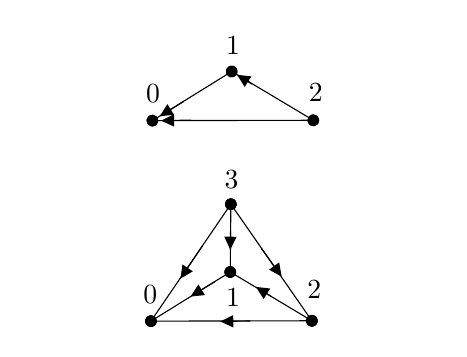
\begin{tikzpicture}[x=0.75pt,y=0.75pt,yscale=-0.7,xscale=0.7]\tikzset{every picture/.style={line width=0.75pt}}

%Straight Lines [id:da31341595090350494] 
\draw    (149.25,245.25) -- (38.5,245.5) ;
\draw [shift={(38.5,245.5)}, rotate = 179.87] [color={rgb, 255:red, 0; green, 0; blue, 0 }  ][fill={rgb, 255:red, 0; green, 0; blue, 0 }  ][line width=0.75]      (0, 0) circle [x radius= 3.35, y radius= 3.35]   ;
\draw [shift={(149.25,245.25)}, rotate = 179.87] [color={rgb, 255:red, 0; green, 0; blue, 0 }  ][fill={rgb, 255:red, 0; green, 0; blue, 0 }  ][line width=0.75]      (0, 0) circle [x radius= 3.35, y radius= 3.35]   ;
%Straight Lines [id:da9609296906616727] 
\draw    (106.88,245.38) -- (88.25,245.71) ;
\draw [shift={(86.25,245.75)}, rotate = 358.96000000000004] [fill={rgb, 255:red, 0; green, 0; blue, 0 }  ][line width=0.75]  [draw opacity=0] (8.93,-4.29) -- (0,0) -- (8.93,4.29) -- cycle    ;

%Straight Lines [id:da252345846123192] 
\draw    (93.5,165) -- (38.5,245.5) ;
\draw [shift={(38.5,245.5)}, rotate = 124.34] [color={rgb, 255:red, 0; green, 0; blue, 0 }  ][fill={rgb, 255:red, 0; green, 0; blue, 0 }  ][line width=0.75]      (0, 0) circle [x radius= 3.35, y radius= 3.35]   ;
\draw [shift={(93.5,165)}, rotate = 124.34] [color={rgb, 255:red, 0; green, 0; blue, 0 }  ][fill={rgb, 255:red, 0; green, 0; blue, 0 }  ][line width=0.75]      (0, 0) circle [x radius= 3.35, y radius= 3.35]   ;
%Straight Lines [id:da11171836378352906] 
\draw    (73.96,193.6) -- (59.88,214.61) ;
\draw [shift={(58.77,216.27)}, rotate = 303.83] [fill={rgb, 255:red, 0; green, 0; blue, 0 }  ][line width=0.75]  [draw opacity=0] (8.93,-4.29) -- (0,0) -- (8.93,4.29) -- cycle    ;

%Straight Lines [id:da9411846809932387] 
\draw    (149.25,245.25) -- (93.5,165) ;
\draw [shift={(93.5,165)}, rotate = 235.21] [color={rgb, 255:red, 0; green, 0; blue, 0 }  ][fill={rgb, 255:red, 0; green, 0; blue, 0 }  ][line width=0.75]      (0, 0) circle [x radius= 3.35, y radius= 3.35]   ;
\draw [shift={(149.25,245.25)}, rotate = 235.21] [color={rgb, 255:red, 0; green, 0; blue, 0 }  ][fill={rgb, 255:red, 0; green, 0; blue, 0 }  ][line width=0.75]      (0, 0) circle [x radius= 3.35, y radius= 3.35]   ;
%Straight Lines [id:da6467035917598132] 
\draw    (114.71,195.71) -- (127.31,213.19) ;
\draw [shift={(128.48,214.81)}, rotate = 234.21] [fill={rgb, 255:red, 0; green, 0; blue, 0 }  ][line width=0.75]  [draw opacity=0] (8.93,-4.29) -- (0,0) -- (8.93,4.29) -- cycle    ;

%Straight Lines [id:da05960945318721844] 
\draw    (93.5,165) -- (93.08,211.67) ;
\draw [shift={(93.08,211.67)}, rotate = 90.51] [color={rgb, 255:red, 0; green, 0; blue, 0 }  ][fill={rgb, 255:red, 0; green, 0; blue, 0 }  ][line width=0.75]      (0, 0) circle [x radius= 3.35, y radius= 3.35]   ;
\draw [shift={(93.5,165)}, rotate = 90.51] [color={rgb, 255:red, 0; green, 0; blue, 0 }  ][fill={rgb, 255:red, 0; green, 0; blue, 0 }  ][line width=0.75]      (0, 0) circle [x radius= 3.35, y radius= 3.35]   ;
%Straight Lines [id:da18779983245814547] 
\draw    (93.08,211.67) -- (38.5,245.5) ;
\draw [shift={(38.5,245.5)}, rotate = 148.21] [color={rgb, 255:red, 0; green, 0; blue, 0 }  ][fill={rgb, 255:red, 0; green, 0; blue, 0 }  ][line width=0.75]      (0, 0) circle [x radius= 3.35, y radius= 3.35]   ;
\draw [shift={(93.08,211.67)}, rotate = 148.21] [color={rgb, 255:red, 0; green, 0; blue, 0 }  ][fill={rgb, 255:red, 0; green, 0; blue, 0 }  ][line width=0.75]      (0, 0) circle [x radius= 3.35, y radius= 3.35]   ;
%Straight Lines [id:da9874513451972009] 
\draw    (93.08,211.67) -- (149.25,245.25) ;
\draw [shift={(149.25,245.25)}, rotate = 30.88] [color={rgb, 255:red, 0; green, 0; blue, 0 }  ][fill={rgb, 255:red, 0; green, 0; blue, 0 }  ][line width=0.75]      (0, 0) circle [x radius= 3.35, y radius= 3.35]   ;
\draw [shift={(93.08,211.67)}, rotate = 30.88] [color={rgb, 255:red, 0; green, 0; blue, 0 }  ][fill={rgb, 255:red, 0; green, 0; blue, 0 }  ][line width=0.75]      (0, 0) circle [x radius= 3.35, y radius= 3.35]   ;
%Straight Lines [id:da21738250880340737] 
\draw    (82.42,218.33) -- (67.49,227.53) ;
\draw [shift={(65.79,228.58)}, rotate = 328.34000000000003] [fill={rgb, 255:red, 0; green, 0; blue, 0 }  ][line width=0.75]  [draw opacity=0] (8.93,-4.29) -- (0,0) -- (8.93,4.29) -- cycle    ;

%Straight Lines [id:da502837847841804] 
\draw    (93.29,183.33) -- (93.13,194.32) ;
\draw [shift={(93.1,196.32)}, rotate = 270.83] [fill={rgb, 255:red, 0; green, 0; blue, 0 }  ][line width=0.75]  [draw opacity=0] (8.93,-4.29) -- (0,0) -- (8.93,4.29) -- cycle    ;

%Straight Lines [id:da38006772268977085] 
\draw    (121.17,228.46) -- (112.46,223) ;
\draw [shift={(110.76,221.94)}, rotate = 392.05] [fill={rgb, 255:red, 0; green, 0; blue, 0 }  ][line width=0.75]  [draw opacity=0] (8.93,-4.29) -- (0,0) -- (8.93,4.29) -- cycle    ;

%Straight Lines [id:da09733860617343582] 
\draw    (150.25,107.25) -- (39.5,107.5) ;
\draw [shift={(39.5,107.5)}, rotate = 179.87] [color={rgb, 255:red, 0; green, 0; blue, 0 }  ][fill={rgb, 255:red, 0; green, 0; blue, 0 }  ][line width=0.75]      (0, 0) circle [x radius= 3.35, y radius= 3.35]   ;
\draw [shift={(150.25,107.25)}, rotate = 179.87] [color={rgb, 255:red, 0; green, 0; blue, 0 }  ][fill={rgb, 255:red, 0; green, 0; blue, 0 }  ][line width=0.75]      (0, 0) circle [x radius= 3.35, y radius= 3.35]   ;
%Straight Lines [id:da9907229664589221] 
\draw    (66.13,107.13) -- (47.5,107.46) ;
\draw [shift={(45.5,107.5)}, rotate = 358.96000000000004] [fill={rgb, 255:red, 0; green, 0; blue, 0 }  ][line width=0.75]  [draw opacity=0] (8.93,-4.29) -- (0,0) -- (8.93,4.29) -- cycle    ;

%Straight Lines [id:da8984506786350759] 
\draw    (94.08,73.67) -- (39.5,107.5) ;
\draw [shift={(39.5,107.5)}, rotate = 148.21] [color={rgb, 255:red, 0; green, 0; blue, 0 }  ][fill={rgb, 255:red, 0; green, 0; blue, 0 }  ][line width=0.75]      (0, 0) circle [x radius= 3.35, y radius= 3.35]   ;
\draw [shift={(94.08,73.67)}, rotate = 148.21] [color={rgb, 255:red, 0; green, 0; blue, 0 }  ][fill={rgb, 255:red, 0; green, 0; blue, 0 }  ][line width=0.75]      (0, 0) circle [x radius= 3.35, y radius= 3.35]   ;
%Straight Lines [id:da13062093153249577] 
\draw    (94.08,73.67) -- (150.25,107.25) ;
\draw [shift={(150.25,107.25)}, rotate = 30.88] [color={rgb, 255:red, 0; green, 0; blue, 0 }  ][fill={rgb, 255:red, 0; green, 0; blue, 0 }  ][line width=0.75]      (0, 0) circle [x radius= 3.35, y radius= 3.35]   ;
\draw [shift={(94.08,73.67)}, rotate = 30.88] [color={rgb, 255:red, 0; green, 0; blue, 0 }  ][fill={rgb, 255:red, 0; green, 0; blue, 0 }  ][line width=0.75]      (0, 0) circle [x radius= 3.35, y radius= 3.35]   ;
%Straight Lines [id:da9384075142317254] 
\draw    (61.13,94.25) -- (46.2,103.45) ;
\draw [shift={(44.5,104.5)}, rotate = 328.34000000000003] [fill={rgb, 255:red, 0; green, 0; blue, 0 }  ][line width=0.75]  [draw opacity=0] (8.93,-4.29) -- (0,0) -- (8.93,4.29) -- cycle    ;

%Straight Lines [id:da2991130569955017] 
\draw    (108.17,82.46) -- (99.46,77) ;
\draw [shift={(97.76,75.94)}, rotate = 392.05] [fill={rgb, 255:red, 0; green, 0; blue, 0 }  ][line width=0.75]  [draw opacity=0] (8.93,-4.29) -- (0,0) -- (8.93,4.29) -- cycle    ;


% Text Node
\draw (94,148) node   {$3$};
% Text Node
\draw (152,88) node   {$2$};
% Text Node
\draw (95,56) node   {$1$};
% Text Node
\draw (151,224) node   {$2$};
% Text Node
\draw (95,229) node   {$1$};
% Text Node
\draw (38,227) node   {$0$};
% Text Node
\draw (40,89) node   {$0$};


\draw (-40,89) node   {};
\draw (230,56) node   {};

\end{tikzpicture}
}\label{subfig-2:von_neu_ord}}
		\caption{\Wf\ sets represented through graphs~\cite{Aczel1989-ACZNS-2}.}
		\label{fig:von_neu_ord}
	\end{figure}
	To formalize this concept of \textquoteleft picture of a set' however it is necessary to introduce the concept of \emph{decoration}:
	%
	\begin{definition} [decoration and picture]
		\begin{itemize}
			\item A \emph{decoration} of a graph \graphVE{V}{E}\ is a function $\delta$ that assigns to each node $\defemph{n} \in V$\ a set $\delta_\defemph{n}$ in such a way that the elements of $\delta_\defemph{n}$ are exactly the sets assigned to successors of \defemph{n}, \ie $\delta_\defemph{n} = \{\delta_\defemph{n^{\prime}} \mid (\defemph{n},\defemph{n}^\prime) \in E\}$.
		
			\item If $\delta$ is a decoration of a pointed graph $(\graphG, \defemph{n})$, then $(\graphG, \defemph{n})$ is a \emph{picture} of the set $\delta_\defemph{n}$.
		\end{itemize}
	\end{definition}
	%
	Moreover, in well-founded set theory, it holds the Mostovski's lemma: \textquotedblleft each \wf\ graph\footnote{A \wf\ graph is a graph that doesn't contain an infinite path $\defemph{n} \rightarrow \defemph{n}^{\prime} \rightarrow \defemph{n}^{\prime\prime} \rightarrow \dots$ of successors.} is a picture of exactly one set".

	
	On the other hand in~\cite{Aczel1989-ACZNS-2} a \emph{\nwf}, or \emph{extraordinary set} in the sense of Mirimanoff, is a set that respects Definition~\ref{def:nwfs}.
	\begin{definition}[\nwf\ set]\label{def:nwfs}
		A set is \emph{\nwf}\ (or \emph{extraordinary}) when among its descents there are some which are infinite.
	\end{definition}
	%
	In fact, when the \textbf{Foundation Axiom}\footnote{Expressed in~\cite{gerbrandy1999bisimulations} as \textquotedblleft Only \wf\ graphs have decorations".} is substituted by the \textbf{Anti-Foundation Axiom} (\textbf{AFA}), expressed by Aczel in~\cite{Aczel1989-ACZNS-2} as \textquotedblleft \textit{Every graph has a unique decoration}", the following consequences become true:
	\begin{itemize}
		%\item Every pointed graph is a picture of a unique set;
			\item Every graph is a picture of exactly one set (\textbf{AFA} as is formulated in~\cite{gerbrandy1999bisimulations});
		\item \nwf\ sets exist given that a \nwf\ pointed graph has to be a picture of a \nwf\ set.
		%\item every graph is a picture of exactly one set (\textbf{AFA} as is formulated in~\cite{gerbrandy1999bisimulations}).
	\end{itemize}
	%
	\begin{figure}
		\centering
		\subfloat[Standard picture $\Omega$.]{\scalebox{0.6}{\input{img/omega}}\label{subfig-omega_nwf:1}}
		\hfill
		\subfloat[Unfolding of the picture of $\Omega$.]{\scalebox{1}{

\tikzset{every picture/.style={line width=0.75pt}} %set default line width to 0.75pt        

\begin{tikzpicture}[x=0.75pt,y=0.75pt,yscale=-1,xscale=1]
%uncomment if require: \path (0,300); %set diagram left start at 0, and has height of 300

%Straight Lines [id:da6276790682079358] 
\draw    (100.6,110) -- (140.85,110) ;


%Flowchart: Connector [id:dp10712755168097865] 
\draw  [fill={rgb, 255:red, 0; green, 0; blue, 0 }  ,fill opacity=1 ] (103,110) .. controls (103,111.33) and (101.93,112.4) .. (100.6,112.4) .. controls (99.27,112.4) and (98.2,111.33) .. (98.2,110) .. controls (98.2,108.67) and (99.27,107.6) .. (100.6,107.6) .. controls (101.93,107.6) and (103,108.67) .. (103,110) -- cycle ;
%Straight Lines [id:da8191358904406301] 
\draw    (139.8,110.2) -- (180.05,110.2) ;


%Flowchart: Connector [id:dp9628511983929124] 
\draw  [fill={rgb, 255:red, 0; green, 0; blue, 0 }  ,fill opacity=1 ] (142.2,110.2) .. controls (142.2,111.53) and (141.13,112.6) .. (139.8,112.6) .. controls (138.47,112.6) and (137.4,111.53) .. (137.4,110.2) .. controls (137.4,108.87) and (138.47,107.8) .. (139.8,107.8) .. controls (141.13,107.8) and (142.2,108.87) .. (142.2,110.2) -- cycle ;
%Shape: Triangle [id:dp18185199166706778] 
\draw  [fill={rgb, 255:red, 0; green, 0; blue, 0 }  ,fill opacity=1 ] (120.72,110) -- (118,111.21) -- (118,108.79) -- cycle ;
%Shape: Triangle [id:dp11767706980455106] 
\draw  [color={rgb, 255:red, 0; green, 0; blue, 0 }  ,draw opacity=1 ][fill={rgb, 255:red, 0; green, 0; blue, 0 }  ,fill opacity=1 ] (159.92,110.2) -- (157.2,111.41) -- (157.2,108.99) -- cycle ;
%Straight Lines [id:da6334935852876922] 
\draw    (180.1,110) -- (220.35,110) ;


%Flowchart: Connector [id:dp022374442404981654] 
\draw  [fill={rgb, 255:red, 0; green, 0; blue, 0 }  ,fill opacity=1 ] (182.5,110) .. controls (182.5,111.33) and (181.43,112.4) .. (180.1,112.4) .. controls (178.77,112.4) and (177.7,111.33) .. (177.7,110) .. controls (177.7,108.67) and (178.77,107.6) .. (180.1,107.6) .. controls (181.43,107.6) and (182.5,108.67) .. (182.5,110) -- cycle ;
%Flowchart: Connector [id:dp8113410302855639] 
\draw  [fill={rgb, 255:red, 0; green, 0; blue, 0 }  ,fill opacity=1 ] (221.7,110.2) .. controls (221.7,111.53) and (220.63,112.6) .. (219.3,112.6) .. controls (217.97,112.6) and (216.9,111.53) .. (216.9,110.2) .. controls (216.9,108.87) and (217.97,107.8) .. (219.3,107.8) .. controls (220.63,107.8) and (221.7,108.87) .. (221.7,110.2) -- cycle ;
%Shape: Triangle [id:dp5972516863295354] 
\draw  [fill={rgb, 255:red, 0; green, 0; blue, 0 }  ,fill opacity=1 ] (200.22,110) -- (197.5,111.21) -- (197.5,108.79) -- cycle ;
%Straight Lines [id:da9015443131541547] 
\draw  [dash pattern={on 0.84pt off 2.51pt}]  (219.3,110.2) -- (250.15,110.2) ;

\draw (250,140) node   {};
\draw (90,140) node   {};


\end{tikzpicture}

}\label{subfig-omega_nwf:2}}
		\caption{Representation of the \nwf\ set $\Omega = \{\Omega\}$~\cite{Aczel1989-ACZNS-2}.}
		\label{fig:omega_nwf}
	\end{figure}


%We can now reformulate \textbf{AFA} as in~\cite{gerbrandy1999bisimulations} to
%	\subsection{Systems of Equations}
%	\Nwf\ sets, as said in \S~\ref{subsec-possibilities:set_th}, can be represented by \nwf\ graphs.
	In~\cite{Aczel1989-ACZNS-2,gerbrandy1999bisimulations} it is pointed out how \nwf\ sets can also be expressed through systems of equations. 
	This concept will help us to formalize the notion of state in our action language.
	
	A quick example of this representation can be derived by the set $\Omega = \{\Omega\}$ (Figure~\ref{fig:omega_nwf}). We can, in fact, informally define this set by the (singleton) system of equations $%\big\{%
	x = \bra{x}$.
	%
	Systems of equations and their solutions are described more formally as follows in~\cite{gerbrandy1999bisimulations}:
	%
	\begin{definition}[system of equations]
		For each class of atoms\footnote{Objects that are not sets and have no further set-theoretic structure.} $\mathcal{X}$ a \emph{system of equation} in $\mathcal{X}$ is a class
		$\tau$ of equations $\poss{x} = \mathtt{X}$, where $\poss{x} \in \mathcal{X}$ and $\mathtt{X} \subseteq \mathcal{X}$, such that  $\tau$ contains exactly one equation $\poss{x} = \mathtt{X}$ for each $\poss{x} \in \mathcal{X}$. 
		%that for each $\poss{x} \in \mathcal{X}$ includes exactly one equation of the form $\poss{x} = \mathtt{X}$ where $\mathtt{X} \subseteq \mathcal{X}$.\\
		A solution to a system of equations $\tau$ is a function $\delta$ that assigns to each $\poss{x} \in \tau(\mathcal{X})$\footnote{$\tau(\mathcal{X})$ denotes the class of atoms $\mathcal{X}$ in which $\tau$ is described.} a set $\delta_\poss{x}$ such that $\delta_\poss{x} = \{ \delta_\defemph{y} \mid \defemph{y} \in \mathtt{X}\}$, where $\poss{x} = \mathtt{X}$ is an equation of $\tau$.
		If $\delta$ is the solution to a system of equations $\tau$, then the set $\{\delta_\poss{x} \mid \poss{x} \in \tau(\mathcal{X})\}$ is called the solution set of that system.
	\end{definition}
	
	Since both  graphs and systems of equations are representations for \nwf\ sets, it is natural to investigate their relationships.
	In particular it is interesting to point out how from a graph \graphVE{V}{E} it is possible to construct a system of equations $\tau$ and vice versa.
	The nodes in $\graphG$, in fact, can be the set of atoms $\tau(\mathcal{X})$ and, for each node $\poss{v} \in V$, an equation  is represented by $ \poss{v} = \{\poss{v}^\prime \mid (\poss{v}, \poss{v}^\prime) \in E\}$.
	Since each graph has a unique decoration, each system of equations has a unique solution.
	This is also true when we consider bisimilar systems of equations. In fact we can collapse them into their minimal representation thanks to the concept of \emph{maximum bisimulation} as introduced in~\cite{DBLP:conf/iclp/Dovier15}.
	Bisimilar labeled graphs (or Kripke structures) have therefore a unique solution as well since we collapse their representations into the minimal one. This idea will be further expanded in Section~\ref{subsec-contribution:bisim}.
	

	
	\subsection{\PosS}\label{subsec-possibilities:possibilities}
	Let us introduce the notion of \pos\, as in~\cite{Gerbrandy1997}:
	\begin{definition}[\posS]\label{def:pos}
		Let \sAG\ be a set of agents and \sP\ a set of propositional variables:%The class of \posS\ is the largest class such that:
		\begin{itemize}
			\item A \emph{\pos}\ $\poss{u}$ is a function that assigns to each propositional variable $\defemph{f} \in \sP$ a truth value $\possarg{u}{\defemph{f}} \in \bra{0,1}$ and to each agent $\agent{ag} \in \sAG$ an information state $\possarg{u}{\agent{ag}} = \sigma$.
			\item An \emph{information state} $\sigma$ is a set of \posS.
		\end{itemize}
	\end{definition}
	
	In Section~\ref{subsec-contribution:state} we will use this concept to describe a \textquoteleft state' of the planning problem.
	The intuition behind this idea is that a \pos\ \poss{u} is a possible interpretation of the world and of the agents' beliefs; in fact $\possarg{u}{\defemph{f}}$ specifies the truth value of the fluent \defemph{f} in \poss{u} and $\possarg{u}{\agent{a}}$ is the set of all the interpretations the agent \agent{a} considers possible in \poss{u}.
	
	Moreover a \pos\ can be pictured as a decoration of a labeled graph and therefore as a unique solution to a system of equations for \posS.
	A \pos\ represents the solution to the minimal system of equations in which all bisimilar systems of equations are collapsed; that is the \posS\ that represent decorations of bisimilar labeled graphs are bisimilar and can be represented by the minimal one.
	This shows that the class of bisimilar labeled graphs and, therefore, of bisimilar Kripke structures, used by \mAL\ as states, can be represented by a single \pos. 
	
	\begin{definition}[equations for \posS] \label{def:soe_poss}
		Given a set of agents \sAG\ and a set of propositional variables \sP, a \emph{system of equations for \posS}\ in a class of \posS\ $\mathcal{X}$ is a set of equations such that for each $\poss{x} \in \mathcal{X}$ there exists exactly one equation of the form $\possarg{x}{\defemph{f}} = i$, where $i \in \bra{0,1}$, for each $\defemph{f} \in \sP$, and of the form $\possarg{x}{\agent{ag}} = \mathtt{X}$, where $\mathtt{X} \subseteq \mathcal{X}$, for each $\agent{ag} \in \sAG$.\\
		A solution to a system of equations for \posS\ is a function $\delta$ that assigns to each atom $\defemph{x}$ a \pos\ $\delta_\poss{x}$ in such a way that if $\possarg{x}{\defemph{f}} = i$ is an equation then $\delta_{\possarg{x}{\defemph{f}}} = i$, and if $\possarg{x}{\agent{ag}} = \sigma$ is an equation, then $\delta_{\possarg{x}{\agent{ag}}} = \bra{\delta_\defemph{y} \mid \defemph{y} \in \sigma}$.
	\end{definition}
%
%	Moreover in~\cite{gerbrandy1999bisimulations} some set based operations on \posS\ are defined . These operations are based on the fact that the class of all \posS\ is the largest fixed point\footnote{The reader is addressed to~\cite{gerbrandy1999bisimulations} for a complete description.} of the set operation $\sPoss(\defemph{\cdot})$:
%	\begin{equation*}
%		\label{page:set_op}
%		\sPoss(S) = \bra{f \mid \text{$f$ is a function } \sP \mapsto \bra{0,1} \cup \sAG \mapsto 2^S}. 
%		%\sPoss(S) = \bra{f \mid \text{$f$: } \sP \mapsto \bra{0,1}} \cup \bra{f \mid \text{$f$: } \sAG \mapsto 2^S} 
%	\end{equation*}
%	
%	Together with corecursion these operations will be used in \S~\ref{subsec-contribution:transfunc} to define the transition function of our language.\todo{Check page 16,17... With prof to ask why corecursion is used that way and how the pump makes our transition function well-defined.}

%\subsubsection{Bisimulation}
%
%

	%
	%
	%
	\section{The action language \ourL} \label{sec:contribution}
	%In this section we introduce \ourL, an action language based on \mAL that, in our opinion, is the most complete action language for epistemic planning in multi-agent domain.\\
		
The research on \mAGep\ domain, both in logic and planning, already comprehends several theoretical studies~\cite{fagin1994reasoning,moore1981reasoning,gerbrandy1999bisimulations,van2008handbook,van1997complete,van2007dynamic,baral2015action,aucher2013undecidability,bolander2015complexity,van2004dynamic} and also a variety of solvers~\cite{kominis2015beliefs,huang2017general,muise2015planning,wan2015complete,liu2018multi,le2018efp} even if, at the best of our knowledge, only~\cite{le2018efp,van2004dynamic} can reason without limitations on domains described by \lagC. 
	
%Given the complexity %(Table~\ref{table:complexity})
%that lies behind reasoning in these domains, it is clear that 
Anyway \mAGep\ solvers still have to reason on domains where the number of fluents and/or agents is limited.
This is to reduce the length of the planning problems solution that otherwise would require an  excessive quantity of resources (\ie time and memory).
For these reasons the demand of computational resources needed (for example in respect to classical planning) is one of the central problem in \mep.
	
To reduce this gap several approaches can be used:
\begin{enumerate*}[label=\roman*)]
	\item as in~\cite{kominis2015beliefs,huang2017general,muise2015planning,wan2015complete} the planning domain can be limited to a less expressive class of problems.
	
	On the other hand, when generality is required, \item heuristics can effectively reduce the resolution process, as shown in~\cite{le2018efp}.
	
	Finally another approach to follow could be \item to consider alternative representations to Kripke structures; this is what \ourL\ tries to do.
\end{enumerate*} 
	
Changing the structure is especially important because different state representation can lead to a better use of the resources, and to exploit properties of the new structure to introduce important functionalities; \eg \ourL\ could rely on the concept of \emph{bisimulation} to introduce the notion of \emph{visited states}, being bisimulation an equality criteria for \nwf\ sets.% \mep\ can be tackled from a different prospective\footnote{In the case of \ourL\ we use a set theoretical approach that introduces the epistemic planning problem to set operations.} and properties of the new structure can be exploited to introduce important functionalities; \eg \ourL\ could rely on the concept of \emph{bisimulation} to introduce the notion of \emph{visited states}, being bisimulation an equality criteria for \nwf\ sets.
	
%\ourL, as already said, is based on \mAL. The difference is in how a state is defined: in fact in \mAL\ a state is represented as Kripke structure while in \ourL\ a state is a \pos\ (for simplicity, we use the same syntax of \mAL).
%
%
%
\subsection{State} \label{subsec-contribution:state}
\FloatBarrier

	As main contribution we introduce a modified version of \mAL, called \ourL. The difference is in how a state is defined: in \mAL\ a state is represented as a Kripke structure while in \ourL\ a state is a \pos\ (\S~\ref{subsec-possibilities:possibilities}). For simplicity, we maintain the syntax used in \mAL.% where a state of the \mep\ problem is represented trough a \pos\ .
	
	The strict connection of these two structures is highlighted in~\cite{gerbrandy1999bisimulations} from the fact that a solution to a system of equations for \posS\ (Definition~\ref{def:soe_poss}) represents a decoration for a labeled graph, which is essentially a Kripke model.
	In~\cite{gerbrandy1999bisimulations}, it is also expressed that a \textquotedblleft \pos\ corresponds with a whole class of bisimilar, but structurally different, Kripke models". 
%	As is not clear what state equality in \mep\ is we leave the formal investigation of whether this structural difference is meaningful in \mep\ as future work.\\ 
	
	Let us define the usage of \posS\ as states in a \mep\ domain where the set of agents is \sAG\ and the set of fluents is \sF.
	A \pos\ %, in the sense of Definition~\ref{def:pos},
	is a function that assigns to each propositional variable $\defemph{f} \in \sF$ a truth value $\possarg{u}{\defemph{f}} \in \bra{0,1}$ and to each agent $\agent{ag} \in \sAG$ a set of \posS\ $\possarg{u}{\agent{ag}}$.
	
	A state in \mep\ has to encode the truth value of the fluents, as in classical planning, and also the beliefs of the agents about fluents and beliefs themselves.
	%In particular an agent that cannot distinguish which world is the real has.
	We defined in \S~\ref{sec:mal} how Kripke structures represent these information.
	In Figure~\ref{fig:state_as_pos} we use a \pos\ as a system of equations to encode a state (of the domain in Example~\ref{ex:coin_box}).
	
	An equation is represented in the form $\poss{u} = \bra{(\agent{ag_1}, \sigma), (\agent{ag_2}, \sigma^\prime), \dots ,\defemph{f}, \defemph{f}^\prime , \dots}$ where \agent{ag_1}, \agent{ag_2} $\in \sAG$, $\sigma, \sigma^\prime$ are sets of \posS\ and $\defemph{f}, \defemph{f}^\prime \in \sF$.
	When we write $ (\agent{ag}, \sigma)$ we mean that, in \poss{u}, the agent \agent{ag} believes that the \posS\ in $\sigma$ are plausible.
	On the other hand only if a fluent $\defemph{f}$ is present in the equation this means that the fluent itself is true in \poss{u}.
	\begin{figure}
		\centering
	%	\hspace*{-4cm}
		\subfloat[System of equations for \posS.]
		{%
			\scalebox{.8}%
			{%
				\raisebox{1.5cm}{
					$\begin{aligned}
	&\begin{cases}
		\emphColorSlide{\poss{w}}&= \bra{
		  	(\agentSlide{ag},\bra{\poss{w}, \poss{w^\prime}}),
		  	(\agentSlide{C},\bra{\poss{v}, \poss{v^\prime}}),
		  	\ttSlide{look(\agentSlide{ag})},
		  	\ttSlide{key(\agentSlide{A})},
		  	\ttSlide{opened},
		  	\ttSlide{heads}%
	  	}\\
		\poss{w^\prime} &=\bra{
		  	(\agentSlide{ag},\bra{\poss{w}, \poss{w^\prime}}),
		  	(\agentSlide{C},\bra{\poss{v}, \poss{v^\prime}}),
		  	\ttSlide{look(\agentSlide{ag})},
		  	\ttSlide{key(\agentSlide{A})}, 
		  	\ttSlide{opened}
	 	 }\\
		\poss{v} &= \bra{
			(\agentSlide{A},\bra{\poss{v}, \poss{v^\prime}}),
			(\agentSlide{B},\bra{\poss{v}, \poss{v^\prime}}),
			(\agentSlide{C},\bra{\poss{v}, \poss{v^\prime}}),
			\ttSlide{look(\agentSlide{ag})},
			\ttSlide{key(\agentSlide{A})},
			\ttSlide{heads}%
		}\\
		\poss{v}^\prime &= \bra{
			(\agentSlide{A},\bra{\poss{v}, \poss{v^\prime}}),
			(\agentSlide{B},\bra{\poss{v}, \poss{v^\prime}}),
			(\agentSlide{C},\bra{\poss{v}, \poss{v^\prime}}),
			\ttSlide{look(\agentSlide{ag})},
			\ttSlide{key(\agentSlide{A})}
		}\\
	\end{cases}\\
	&\text{where }\agentSlide{ag} \in \bra{\agentSlide{A}, \agentSlide{B}}.
\end{aligned}$



				}%
			}%
			\label{subfig-state_as_pos:1}
		}%
		%\hspace*{.5cm}
		\subfloat[Decoration of the pointed labeled graph $(\graphG, \poss{w})$.]
		{% 
			\scalebox{0.7}%
			{%
				\raisebox{0cm}{
					

\tikzset{every picture/.style={line width=0.75pt}} %set default line width to 0.75pt        
\trimbox{0cm 0cm 0cm 1.8cm}{ 

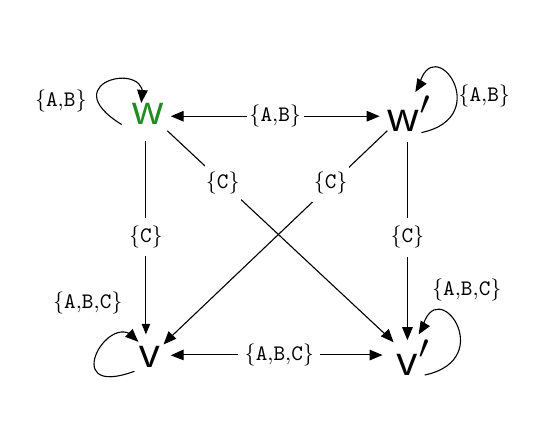
\begin{tikzpicture}[x=0.75pt,y=0.75pt,yscale=-1,xscale=1]
%uncomment if require: \path (0,237.1999969482422); %set diagram left start at 0, and has height of 237.1999969482422

%Straight Lines [id:da49380865843539024] 
\draw    (58,37.52) -- (58,129.88) ;


%Curve Lines [id:da5900505897070274] 
\draw    (55.82,18.4) .. controls (62.62,-2.4) and (11.9,8.32) .. (46.3,29.52) ;


%Shape: Triangle [id:dp7638941010979212] 
\draw  [fill={rgb, 255:red, 0; green, 0; blue, 0 }  ,fill opacity=1 ] (55.82,18.4) -- (54.11,12.94) -- (58.52,13.35) -- cycle ;
%Curve Lines [id:da33896708594278424] 
\draw    (53.81,133.72) .. controls (41.67,115.51) and (14.49,162.32) .. (52.43,148.41) ;


%Shape: Triangle [id:dp06181068467144124] 
\draw  [fill={rgb, 255:red, 0; green, 0; blue, 0 }  ,fill opacity=1 ] (53.81,133.72) -- (48.46,131.68) -- (51.51,128.48) -- cycle ;
%Straight Lines [id:da3518787636435954] 
\draw    (73.3,140.52) -- (171.3,140.52) ;


%Straight Lines [id:da9419961743422685] 
\draw    (167.3,25.52) -- (73.3,25.52) ;


%Straight Lines [id:da5282217469281014] 
\draw    (184,37.72) -- (184,130.08) ;


%Curve Lines [id:da1255493565606156] 
\draw    (191.12,127.8) .. controls (197.84,99.92) and (228.32,142.6) .. (192.32,150.2) ;


%Shape: Triangle [id:dp330887907957337] 
\draw  [fill={rgb, 255:red, 0; green, 0; blue, 0 }  ,fill opacity=1 ] (189.76,130.06) -- (190.59,124.4) -- (194.38,126.68) -- cycle ;
%Curve Lines [id:da19283464821040464] 
\draw    (189.52,11) .. controls (196.24,-16.88) and (226.72,25.8) .. (190.72,33.4) ;


%Shape: Triangle [id:dp48172892570830794] 
\draw  [fill={rgb, 255:red, 0; green, 0; blue, 0 }  ,fill opacity=1 ] (188.16,13.26) -- (188.99,7.6) -- (192.78,9.88) -- cycle ;
%Shape: Triangle [id:dp06884054633092584] 
\draw  [fill={rgb, 255:red, 0; green, 0; blue, 0 }  ,fill opacity=1 ] (184,132.72) -- (181.79,127.43) -- (186.21,127.44) -- cycle ;
%Shape: Triangle [id:dp349860096054311] 
\draw  [fill={rgb, 255:red, 0; green, 0; blue, 0 }  ,fill opacity=1 ] (171.3,140.58) -- (166.02,142.79) -- (166.02,138.37) -- cycle ;
%Shape: Triangle [id:dp5271852980265475] 
\draw  [fill={rgb, 255:red, 0; green, 0; blue, 0 }  ,fill opacity=1 ] (70.66,140.7) -- (75.94,138.31) -- (75.94,142.73) -- cycle ;
%Shape: Triangle [id:dp36308950352931935] 
\draw  [fill={rgb, 255:red, 0; green, 0; blue, 0 }  ,fill opacity=1 ] (58,129.88) -- (56.3,125.81) -- (59.7,125.81) -- cycle ;
%Shape: Triangle [id:dp1292227483684376] 
\draw  [fill={rgb, 255:red, 0; green, 0; blue, 0 }  ,fill opacity=1 ] (70.66,25.52) -- (75.94,23.31) -- (75.94,27.73) -- cycle ;
%Shape: Triangle [id:dp08607057312201727] 
\draw  [fill={rgb, 255:red, 0; green, 0; blue, 0 }  ,fill opacity=1 ] (169.94,25.52) -- (164.66,27.73) -- (164.66,23.31) -- cycle ;
%Straight Lines [id:da22782472852235425] 
\draw    (68.3,32.51) -- (176.84,133.88) ;


%Straight Lines [id:da40972295623496247] 
\draw    (174.3,32.51) -- (68.8,133.01) ;


%Shape: Triangle [id:dp9557525693039122] 
\draw  [fill={rgb, 255:red, 0; green, 0; blue, 0 }  ,fill opacity=1 ] (176.84,133.88) -- (171.64,131.49) -- (174.89,128.49) -- cycle ;
%Shape: Triangle [id:dp9360830131568407] 
\draw  [fill={rgb, 255:red, 0; green, 0; blue, 0 }  ,fill opacity=1 ] (66.99,134.94) -- (69,129.58) -- (72.22,132.61) -- cycle ;

% Text Node
\draw (59,24.32) node [scale=1.7280000000000002] [align=left] {\emphColorSlide{\poss{w}}};
% Text Node
\draw (59.8,141.22) node [scale=1.7280000000000002] [align=left] {\poss{v}};
% Text Node
\draw (17,18.32) node [scale=0.8] [align=left] {\{\agentSlide{A},\agentSlide{B}\}};
% Text Node
\draw (30,115.32) node [scale=0.8] [align=left] {\{\agentSlide{A},\agentSlide{B},\agentSlide{C}\}};
% Text Node
\draw (185.2,24.32) node [scale=1.7280000000000002] [align=left] {\poss{w'}};
% Text Node
\draw (187.11,141.72) node [scale=1.7280000000000002] [align=left] {\poss{v'}};
% Text Node
\draw (212.6,109.32) node [scale=0.8] [align=left] {\{\agentSlide{A},\agentSlide{B},\agentSlide{C}\}};
% Text Node
\draw (221,15.52) node [scale=0.8] [align=left] {\{\agentSlide{A},\agentSlide{B}\}};
% Text Node
\draw  [color={rgb, 255:red, 255; green, 255; blue, 255 }  ,draw opacity=1 ][fill={rgb, 255:red, 255; green, 255; blue, 255 }  ,fill opacity=1 ]  (106.8,16.52) -- (133.8,16.52) -- (133.8,34.52) -- (106.8,34.52) -- cycle  ;
\draw (120.3,25.52) node [scale=0.8,color={rgb, 255:red, 0; green, 0; blue, 0 }  ,opacity=1 ] [align=left] {\{\agentSlide{A},\agentSlide{B}\}};
% Text Node
\draw  [color={rgb, 255:red, 255; green, 255; blue, 255 }  ,draw opacity=1 ][fill={rgb, 255:red, 255; green, 255; blue, 255 }  ,fill opacity=1 ]  (49.5,74.7) -- (66.5,74.7) -- (66.5,92.7) -- (49.5,92.7) -- cycle  ;
\draw (58,83.7) node [scale=0.8,color={rgb, 255:red, 0; green, 0; blue, 0 }  ,opacity=1 ] [align=left] {\{\agentSlide{C}\}};
% Text Node
\draw  [color={rgb, 255:red, 255; green, 255; blue, 255 }  ,draw opacity=1 ][fill={rgb, 255:red, 255; green, 255; blue, 255 }  ,fill opacity=1 ]  (175.5,74.9) -- (192.5,74.9) -- (192.5,92.9) -- (175.5,92.9) -- cycle  ;
\draw (184,83.9) node [scale=0.8,color={rgb, 255:red, 0; green, 0; blue, 0 }  ,opacity=1 ] [align=left] {\{\agentSlide{C}\}};
% Text Node
\draw  [color={rgb, 255:red, 255; green, 255; blue, 255 }  ,draw opacity=1 ][fill={rgb, 255:red, 255; green, 255; blue, 255 }  ,fill opacity=1 ]  (86.5,48.7) -- (103.5,48.7) -- (103.5,66.7) -- (86.5,66.7) -- cycle  ;
\draw (95,57.7) node [scale=0.8,color={rgb, 255:red, 0; green, 0; blue, 0 }  ,opacity=1 ] [align=left] {\{\agentSlide{C}\}};
% Text Node
\draw  [color={rgb, 255:red, 255; green, 255; blue, 255 }  ,draw opacity=1 ][fill={rgb, 255:red, 255; green, 255; blue, 255 }  ,fill opacity=1 ]  (138.5,48.7) -- (155.5,48.7) -- (155.5,66.7) -- (138.5,66.7) -- cycle  ;
\draw (147,57.7) node [scale=0.8,color={rgb, 255:red, 0; green, 0; blue, 0 }  ,opacity=1 ] [align=left] {\{\agentSlide{C}\}};
% Text Node
\draw  [color={rgb, 255:red, 255; green, 255; blue, 255 }  ,draw opacity=1 ][fill={rgb, 255:red, 255; green, 255; blue, 255 }  ,fill opacity=1 ]  (102.8,131.52) -- (141.8,131.52) -- (141.8,149.52) -- (102.8,149.52) -- cycle  ;
\draw (122.3,140.52) node [scale=0.8,color={rgb, 255:red, 0; green, 0; blue, 0 }  ,opacity=1 ] [align=left] {\{\agentSlide{A},\agentSlide{B},\agentSlide{C}\}};


\end{tikzpicture}
}

				}%
			}%
			\label{subfig-state_as_pos:2}%
		}
		\caption{Representation of the possibility \poss{w} after the execution of the actions \distract{C}{A};\open{A} on the initial state of Example~\ref{ex:coin_box}. The \pos\ is expanded to its system of equation for clarity.}
		\label{fig:state_as_pos}
	\end{figure}%
%	

	It is clear that a \pos\ correspond to a decoration of a pointed labeled graph and therefore to a unique Kripke model up to bisimulation.
	The representation through \posS\ allows, in our opinion, a more clear and concise view of the state. That is because each state is represented by a single \pos;
	\eg Figure~\ref{fig:state_as_pos} is represented by \poss{w}= \bra{(\agent{ag},\bra{\poss{w}, \poss{w^\prime}}),(\agent{c},\bra{\poss{v}, \poss{v^\prime}}),\looking{ag},\haskey{a},\opened} where \agent{ag} $\in \bra{\agent{A}, \agent{B}}$.
%
%
%
\FloatBarrier
\subsection{State equality through Bisimulation} \label{subsec-contribution:bisim}
\FloatBarrier

	One of the reasons we chose to use \posS\ as states is to exploit this new structure to introduce new functionalities to \mep.
	In fact having the states described as \posS, which are strongly related to \nwf\ sets, help us to introduce the concept of \emph{visited states}, a core idea in planning.
	
	As said before, a \pos\ in the sense of decoration, represents all the Kripke structures bisimilar to the decoration itself.
	This means that with \posS\ we can exploit bisimulation to capture the idea of equality between states.
	In fact, given two bisimilar decorations (or labeled graphs), these, even with structural differences, are represented by the same \pos.
	On the other hand this is not true when it comes to Kripke structures.
	This idea is best described through  graphical representation; therefore we will use Figure~\ref{fig:equality} to explain this concept.
	
	As an example, let us introduce two  new actions: \flip{} and \tell{ag}{}.
	The first one is an ontic action, where an agent inverts the position of the coin; the observability of this action depends on the fluents \texttt{looking}.
	On the other hand, \tell{ag}{} means that an agent announces to \agent{ag} the position in which she thinks the coin lies while all the other agents are oblivious.
	
	Assuming that the coin lies tails up and given a sequence of action instances $\Delta = \peek{B};\distract{B}{C};\flip{C};\tell{B}{C}$\footnote{We recall that in \cite{baral2015action} an action instance is represented as $\mathtt{action}\tuple{\agent{ag}}$ where \agent{ag} is the agent that executes $\mathtt{action}$.} we show in Figure~\ref{subfig-complete:equality} the result of applying $\Delta$ in a slightly modified initial state of Example~\ref{ex:coin_box} where $\C_{\bra{A,B,C}}$(\opened\ $\wedge \neg \looking{A}$).
	In Figure~\ref{subfig-reduced:equality}, it is represented a Kripke structure that has structural differences in respect to the one in Figure~\ref{subfig-complete:equality}. This means that these two Kripke structures represent two different states in \mAL\ even if they are intuitively the same.
	On the contrary, if we think in term of \posS, both the Kripke structures of Figure~\ref{fig:equality} are represented by \pos\ \begin{center}
  \poss{r_1}=\bra{
    (\agentSlide{A}, \bra{\poss{s_0}, \poss{s_1}}),
    (\agentSlide{B}, \bra{\poss r_1}),
    (\agentSlide{C}, \bra{\poss r_1}),
    \ttSlide{look(\agentSlide{C})},
    \ttSlide{key(\agentSlide{A})},
	\ttSlide{opened},
	\ttSlide{heads}
}
\end{center}

	
	\begin{figure}
		\centering
		\subfloat[The resulting Kripke structure after the execution of $\Delta$.]{\scalebox{.4}{\input{img/equality1_corr}}\label{subfig-complete:equality}}
		\hfill
		\subfloat[A Kripke structure bisimilar to the one in Figure~\ref{subfig-complete:equality}.]{\scalebox{0.4}{\tikzset{every picture/.style={line width=0.75pt}} %set default line width to 0.75pt        
\trimbox{0cm 0cm 0cm 1.8cm}{ 
\begin{tikzpicture}[x=0.75pt,y=0.75pt,yscale=-1,xscale=1]
%uncomment if require: \path (0,332); %set diagram left start at 0, and has height of 332

%Shape: Circle [id:dp09506861109760789] 
\draw   (67.5,279.5) .. controls (67.5,262.66) and (81.16,249) .. (98,249) .. controls (114.84,249) and (128.5,262.66) .. (128.5,279.5) .. controls (128.5,296.34) and (114.84,310) .. (98,310) .. controls (81.16,310) and (67.5,296.34) .. (67.5,279.5) -- cycle ;
%Shape: Circle [id:dp3674876277032001] 
\draw   (240.5,279.5) .. controls (240.5,262.66) and (254.16,249) .. (271,249) .. controls (287.84,249) and (301.5,262.66) .. (301.5,279.5) .. controls (301.5,296.34) and (287.84,310) .. (271,310) .. controls (254.16,310) and (240.5,296.34) .. (240.5,279.5) -- cycle ;
%Straight Lines [id:da686791560478396] 
\draw    (131,279.5) -- (238.5,279.5) ;
\draw [shift={(240.5,279.5)}, rotate = 180] [fill={rgb, 255:red, 0; green, 0; blue, 0 }  ][line width=0.75]  [draw opacity=0] (8.93,-4.29) -- (0,0) -- (8.93,4.29) -- cycle    ;
\draw [shift={(129,279.5)}, rotate = 0] [fill={rgb, 255:red, 0; green, 0; blue, 0 }  ][line width=0.75]  [draw opacity=0] (8.93,-4.29) -- (0,0) -- (8.93,4.29) -- cycle    ;
%Curve Lines [id:da3133467592132765] 
\draw    (67.5,279.5) .. controls (-31.5,263.58) and (50.67,180.83) .. (89.42,247.48) ;
\draw [shift={(90,248.5)}, rotate = 240.66] [fill={rgb, 255:red, 0; green, 0; blue, 0 }  ][line width=0.75]  [draw opacity=0] (8.93,-4.29) -- (0,0) -- (8.93,4.29) -- cycle    ;

%Curve Lines [id:da09866336174690571] 
\draw    (301.5,279.5) .. controls (391.91,267.58) and (313.16,179.07) .. (280.98,249.43) ;
\draw [shift={(280.5,250.5)}, rotate = 293.78] [fill={rgb, 255:red, 0; green, 0; blue, 0 }  ][line width=0.75]  [draw opacity=0] (8.93,-4.29) -- (0,0) -- (8.93,4.29) -- cycle    ;

%Shape: Circle [id:dp9019764791073822] 
\draw  [fill={rgb, 255:red, 0; green, 0; blue, 0 }  ,fill opacity=1 ] (240.5,73.5) .. controls (240.5,56.66) and (254.16,43) .. (271,43) .. controls (287.84,43) and (301.5,56.66) .. (301.5,73.5) .. controls (301.5,90.34) and (287.84,104) .. (271,104) .. controls (254.16,104) and (240.5,90.34) .. (240.5,73.5) -- cycle ;
%Shape: Circle [id:dp23164546006052256] 
\draw  [fill={rgb, 255:red, 255; green, 255; blue, 255 }  ,fill opacity=1 ] (246,73.5) .. controls (246,59.69) and (257.19,48.5) .. (271,48.5) .. controls (284.81,48.5) and (296,59.69) .. (296,73.5) .. controls (296,87.31) and (284.81,98.5) .. (271,98.5) .. controls (257.19,98.5) and (246,87.31) .. (246,73.5) -- cycle ;
%Straight Lines [id:da3406951202857561] 
\draw    (255.5,96.5) -- (112.48,251.28) ;
\draw [shift={(111.13,252.75)}, rotate = 312.74] [fill={rgb, 255:red, 0; green, 0; blue, 0 }  ][line width=0.75]  [draw opacity=0] (8.93,-4.29) -- (0,0) -- (8.93,4.29) -- cycle    ;

%Straight Lines [id:da5969218919849798] 
\draw    (271,104) -- (271,247) ;
\draw [shift={(271,249)}, rotate = 270] [fill={rgb, 255:red, 0; green, 0; blue, 0 }  ][line width=0.75]  [draw opacity=0] (8.93,-4.29) -- (0,0) -- (8.93,4.29) -- cycle    ;

%Curve Lines [id:da32162073734028385] 
\draw    (296.5,72.5) .. controls (386.91,60.58) and (308.16,-27.93) .. (275.98,42.43) ;
\draw [shift={(275.5,43.5)}, rotate = 293.78] [fill={rgb, 255:red, 0; green, 0; blue, 0 }  ][line width=0.75]  [draw opacity=0] (8.93,-4.29) -- (0,0) -- (8.93,4.29) -- cycle    ;


% Text Node
\draw  [color={rgb, 255:red, 255; green, 255; blue, 255 }  ,draw opacity=1 ][fill={rgb, 255:red, 255; green, 255; blue, 255 }  ,fill opacity=1 ]  (155.75,267.5) -- (213.75,267.5) -- (213.75,291.5) -- (155.75,291.5) -- cycle  ;
\draw (184.75,279.5) node   {\{\agentSlide{A},\agentSlide{B},\agentSlide{C}\}};
% Text Node
\draw (98,279.5) node   {\defemph{s_{0}}};
% Text Node
\draw (271,279.5) node   {\defemph{s_{1}}};
% Text Node
\draw  [color={rgb, 255:red, 255; green, 255; blue, 255 }  ,draw opacity=1 ][fill={rgb, 255:red, 255; green, 255; blue, 255 }  ,fill opacity=1 ]  (16,219.5) -- (74,219.5) -- (74,243.5) -- (16,243.5) -- cycle  ;
\draw (45,231.5) node   {\{\agentSlide{A},\agentSlide{B},\agentSlide{C}\}};
% Text Node
\draw  [color={rgb, 255:red, 255; green, 255; blue, 255 }  ,draw opacity=1 ][fill={rgb, 255:red, 255; green, 255; blue, 255 }  ,fill opacity=1 ]  (290,214.5) -- (348,214.5) -- (348,238.5) -- (290,238.5) -- cycle  ;
\draw (319,226.5) node   {\{\agentSlide{A},\agentSlide{B},\agentSlide{C}\}};
% Text Node
\draw (271,73.5) node   {\defemph{r_{1}}};
% Text Node
\draw  [color={rgb, 255:red, 255; green, 255; blue, 255 }  ,draw opacity=1 ][fill={rgb, 255:red, 255; green, 255; blue, 255 }  ,fill opacity=1 ]  (217.5,112.5) -- (238.5,112.5) -- (238.5,136.5) -- (217.5,136.5) -- cycle  ;
\draw (228,124.5) node   {\{\agentSlide{A}\}};
% Text Node
\draw  [color={rgb, 255:red, 255; green, 255; blue, 255 }  ,draw opacity=1 ][fill={rgb, 255:red, 255; green, 255; blue, 255 }  ,fill opacity=1 ]  (261,130.5) -- (282,130.5) -- (282,154.5) -- (261,154.5) -- cycle  ;
\draw (271.5,142.5) node   {\{\agentSlide{A}\}};
% Text Node
\draw  [color={rgb, 255:red, 255; green, 255; blue, 255 }  ,draw opacity=1 ][fill={rgb, 255:red, 255; green, 255; blue, 255 }  ,fill opacity=1 ]  (321,22.5) -- (359,22.5) -- (359,46.5) -- (321,46.5) -- cycle  ;
\draw (340,34.5) node   {\{\agentSlide{B},\agentSlide{C}\}};


\end{tikzpicture}}}\label{subfig-reduced:equality}}
		%
		%\subfloat[Alternative Pictures of Von Neumann ordinals 2 and 3.]{\scalebox{1}{\begin{center}
  \poss{r_1}=\bra{
    (\agentSlide{A}, \bra{\poss{s_0}, \poss{s_1}}),
    (\agentSlide{B}, \bra{\poss r_1}),
    (\agentSlide{C}, \bra{\poss r_1}),
    \ttSlide{look(\agentSlide{C})},
    \ttSlide{key(\agentSlide{A})},
	\ttSlide{opened},
	\ttSlide{heads}
}
\end{center}
}\label{subfig-soe:equality}}
		%
		\caption{Bisimilar Kripke Structures.}
		\label{fig:equality}
	\end{figure}
        %Even if it is not clear whether two different \posS\ may encode the same epistemic properties (we leave this problem for future works) t
        Thanks to the use
        of \posS\ we can capture bisimilar decoration while the same were considered different in \mAL\ and, therefore, check if a state has already been visited. 
%	It also interesting to notice that, since \posS\ are described in a set-based environment, operations on sets
	%, as we will see in \S~\ref{subsec-contribution:transfunc},
%	can be exploited to define the concept of update.
	Next we define the concept of entailment and finally the transition function in \ourL.
%
%
%
\FloatBarrier
\subsection{Entailment} \label{subsec-contribution:entail}
	
%	We firstly give a definition of entailment that resemble the one of \mAL\ (\S~\ref{sec:mal}); the difference lies, as said before, in the fact that \mAL\ bases its entailment on Kripke structures while \ourL\ defines its on \posS.
	%The concept of entailment also connected to the axiomatization proposed in Subsection 4.4 of~\cite{gerbrandy1999bisimulations}.
	
	We now %first of all 
	introduce the
	concept of entailment w.r.t. \posS.
	% (in the sense of Definition~\ref{def:fluent_formula}).
	
		\begin{definition}[entailment w.r.t. \posS]\label{def:poss_truth_fluent}
		Given the belief formulae
	$\varphi,\varphi_{1},\varphi_{2}$, a fluent \defemph{f}, an agent \agent{ag}, a group of agents $\alpha$, and a \pos\ \poss{u}:
		\begin{enumerate}[label= \emph{(}\roman*\emph{)}]
			\item $\poss{u} \models \defemph{f}$ if $\possarg{u}{\defemph{f}}= 1$;
		%	\item $\poss{u} \models \neg \defemph{f}$ if $\possarg{u}{\defemph{f}} = 0$;
			\item $\poss{u} \models \neg \phi$ if $\poss{u} \not \models \phi$;
			\item $\poss{u} \models \phi_1 \vee \phi_2$ if $\poss{u} \models
			\phi_1$ or $\poss{u} \models \phi_2$;
			\item $\poss{u} \models \phi_1 \wedge \phi_2$ if $\poss{u} \models
			\phi_1$ and $\poss{u} \models \phi_2$.
	%		\item $\poss{u} \models \varphi$ accordingly to \emph{Definition~\ref{def:poss_truth_fluent}} if $\varphi$ is a fluent formula;
			\item $\poss{u} \models \bB{ag}{\varphi}$ if for each $\poss{v} \in \possarg{u}{\agent{ag}}$, $\poss{v} \models \varphi$;%\footnote{The transitive closure is assured by the fact that when we reason with beliefs we guarantee that $\forall \varphi, \psi\in \lagC:
			%	M \models ( \bB{ag}{\varphi} \wedge  \bB{ag}{(\varphi \implies \psi)})
			%	\implies \bB{ag}{\psi}$ (what is called property \textbf{K} in Kripke structures).};
			\item $\poss{u} \models \neg \varphi$ if $\poss{u} \not\models \varphi$;
			\item $\poss{u} \models \varphi_1 \vee \varphi_2$ if $\poss{u} \models \varphi_1$ or $\poss{u}\models \varphi_2$;
			\item $\poss{u} \models \varphi_1 \wedge \varphi_2$ if $\poss{u} \models \varphi_1$ and $\poss{u}\models \varphi_2$;
			\item $\poss{u} \models \eAlpha{\varphi}$ if $\poss{u} \models
			\bB{ag}{\varphi}$ for all $\agent{ag} \in \alpha$;
%			\item[\emph{(}xi$^*$\emph{)}] $\poss{u} \models \eAlpha{\varphi}$ if $\bigcup_{\agent{ag} \in \alpha} \possarg{u}{\agent{ag}} \models \varphi$;
			\item $\poss{u} \models \cAlpha{\varphi}$ if
			$\poss{u} \models \eAlphaIter{k}{\varphi}$ for every
			$k\geq0$, where $\eAlphaIter{0}{\varphi} = \varphi$ and
			$\eAlphaIter{k+1}{\varphi}=\eAlpha{(\eAlphaIter{k}{\varphi})}$.
		\end{enumerate}
	\end{definition}

	%The operator \E\ can be restated through the set operation $\cup$:
%	\todo{Ask to prof} As the correctness and completeness of this transition function is not yet demonstrated we just present the description of the function with a brief comment on the intuition that lies behind it.
%
%
%
\subsection{Transition function} \label{subsec-contribution:transfunc}
	Finally we introduce the transition function for \ourL.
	%The transition function is based on the concept of corecursion as expressed in Subsection~1.2 of~\cite{gerbrandy1999bisimulations}. In fact, as we said in \S~\ref{subsec-possibilities:possibilities}, the class of all the \posS\ is the largest fixed point of the operator introduced in Page~\pageref{page:set_op}.
	In defining this transition function we made some assumptions:
	\begin{enumerate*}[label=\roman*)]
		\item we consider that the given initial state also specifies which world is the pointed one (as said in~\cite{baral2015action}), this allow us to relax the description of $\Phi$ in the case of announcements or sensing actions.

		Moreover \item we do not take into consideration the case in which an agent can have \emph{false beliefs}\footnote{An agent \agent{ag} has a false belief about $\varphi$ in state \defemph{s} if \defemph{s} $\models \varphi$ and \defemph{s} $\models \bB{ag}{\neg \varphi}$.} because is still an open question how to deal with them in \mep; we will try to address this problem in future works.
	\end{enumerate*} 
	The transition function relative to the domain \emph{D} is $\trfunc: \ai\times\Sigma \rightarrow \Sigma \cup \bra{\emptyset}$ where $\Sigma$ is the set of all the \posS.
	
	For the sake of readability, the abbreviations used in the following definition are explained at the end of it.
	\begin{definition}[transition function for \ourL]
		Let \defemph{a} $\in \ai$, and a \pos\ \poss{u} be given.
		If \defemph{a} is not executable in \poss{u} then\ $\trfunc(\defemph{a}, \poss{u}) =  \emptyset$
		otherwise if \defemph{a} is executable in \poss{u} :
		\begin{itemize}
			\item $\trfunc( \defemph{a}, \poss{u}) = \poss{v} \text{ if \defemph{a} is an ontic action instance and }$\\
			%	\begin{itemize}
			%	\item
				$\begin{cases}
					\possarg{v}{\defemph{f}} = \possarg{u}{\defemph{f}} &\text{ if } \defemph{f} \neq \res{a}\\
					\possarg{v}{\defemph{f}} = \res{a} &\text{ if } \defemph{f} = \res{a}
					%\res a &\text{ if } \defemph{f} \in \res{a}
				\end{cases}$
				\vspace*{0.1cm}
				\\and
				\vspace*{0.1cm}
				\\
				$\begin{cases}
					\possarg{v}{\agent{ag}} = \possarg{u}{\agent{ag}} &\text{ if } \agent{ag} \in \posoblivious\\
					\possarg{v}{\agent{ag}} = \bigcup_{\poss{w} \in \possarg{u}{\agent{ag}}} \trfunc( \defemph{a}, \poss{w}) &\text{ if } \agent{ag} \in \posfull			
				\end{cases}$
				\vspace*{0.3cm}
			%	\end{itemize}
			\item $\trfunc( \defemph{a}, \poss{u}) = \poss{v} \text{ if \defemph{a} sensed the fluent \defemph{f} }$\\
			%	\begin{itemize}
				%	\item
				$\begin{cases}
							%\trfunc( \defemph{a}, \poss{v}) \text{ s.t. } \poss{v} \in \possarg{u}{\agent{ag}} &\text{ if } \sensed{a}{f} \neq \possarg{u}{\defemph{f}}\\
					\emptyset &\text{ if } \sensed{a}{f} \neq \possarg{u}{\defemph{f}}\\
					\possarg{v}{\agent{ag}} = \possarg{u}{\agent{ag}} &\text{ if } \agent{ag} \in \posoblivious \text{ and } \sensed{a}{f} = \possarg{u}{\defemph{f}}\\
					\possarg{v}{\agent{ag}} = \bigcup_{\poss{w} \in \possarg{u}{\agent{ag}}} \trfunc( \defemph{a}, \poss{w}) &\text{ if }\agent{ag} \in \posfull \text{ and } \sensed{a}{f} = \possarg{u}{\defemph{f}}\\
					\possarg{v}{\agent{ag}} = \bigcup_{\poss{w} \in \possarg{u}{\agent{ag}}} (\trfunc( \defemph{a}, \poss{w}) \cup \trfunc( \neg\defemph{a}, \poss{w})) &\text{ if }\agent{ag} \in \pospartial \text{ and } \sensed{a}{f} = \possarg{u}{\defemph{f}}
				\end{cases}$
				\vspace*{0.3cm}
			%	\end{itemize}
			\item $\trfunc( \defemph{a}, \poss{u}) = \poss{v} \text{ if \defemph{a} announces the fluent formula $\phi$ }$\\
			%	\begin{itemize}
			%		\item
				$\begin{cases}
					%\trfunc( \defemph{a}, \poss{v}) \text{ s.t. } \poss{v} \in \possarg{u}{\agent{ag}} &\text{ if } \sensed{a}{f} \neq \possarg{u}{\defemph{f}}\\
					\emptyset &\text{ if } \poss{u} \not \models \phi\\
					\possarg{v}{\agent{ag}} = \possarg{u}{\agent{ag}} &\text{ if } \agent{ag} \in \posoblivious \text{ and } \poss{u} \models \phi\\
					\possarg{v}{\agent{ag}} = \bigcup_{\poss{w} \in \possarg{u}{\agent{ag}}} \trfunc( \defemph{a}, \poss{w}) &\text{ if } \agent{ag} \in \posfull \text{ and } \poss{u} \models \phi\\
					\possarg{v}{\agent{ag}} = \bigcup_{\poss{w} \in \possarg{u}{\agent{ag}}} (\trfunc( \defemph{a}, \poss{w}) \cup \trfunc( \neg\defemph{a}, \poss{w})) &\text{ if }\agent{ag} \in \pospartial \text{ and } \poss{u} \models \phi
				\end{cases}$
			%	\end{itemize}
		\end{itemize}
			
	\end{definition}
	{\footnotesize 
		where:
	\begin{itemize}
		\item \res{a} is the fluent modified by the action instance \defemph{a};
		
		\item \posfull, \pospartial, \posoblivious\ identify the fully observant, partially observant and oblivious agents respectively;
			
		\item \sensed{a}{f} represents the truth value of the fluent \defemph{f} determined by \defemph{a} = \possarg{u}{\defemph{f}};
			
		\item $\neg\defemph{a}$ describes the action that senses the opposite of \defemph{a}; namely \sensed{a}{\neg f}.
	\end{itemize}}
%
Note that sensing and announcement actions generate the empty set when the action effects do not respect the fluents truth values of the possibility where the action is executed. That is because epistemic action (\ie announcement or sensing) cannot change the state of the world but only the beliefs of the agent.

As example we present the execution of the sequence \distract{C}{A}; \open{A} on the initial state of Example~\ref{ex:coin_box} encoded by the \pos\ \poss{u} in Figure~\ref{subfig-our_tra_func:initial}.
	\begin{figure}
		\centering
		\subfloat[The initial state \poss{u}.]
		{% 
			\scalebox{0.95}%
			{%
					$\begin{cases}
 \poss u &= \bra{(\agent{ag},\bra{\poss{u}, \poss{u^\prime}}), \looking{ag}, \haskey{a}}\\
 \poss u^\prime &= \bra{(\agent{ag},\bra{\poss{u}, \poss{u^\prime}}), \looking{ag}, \haskey{a}, \head}
\end{cases}$

			}%
			\label{subfig-our_tra_func:initial}%
		}
		\subfloat[The state \poss{v} after executing \distract{C}{A}.]
		{%
			\scalebox{0.95}%
			{%
				$\begin{cases}
		\poss{v}&= \bra{
	     	(\agent{ag},\bra{\poss{v}, \poss{v^\prime}}),	\looking{a},
	     	\looking{b},
	     	\haskey{a}%
		}\\
			\poss{v}^\prime&= \bra{
	    	(\agent{ag},\bra{\poss{v}, \poss{v^\prime}}),
	    	\looking{a},
	    	\looking{b},
	    	\haskey{a},
	    	\head%
		}\\
\end{cases}$



			}%
			\label{subfig-our_tra_func:distract}%
		}
			\hfill	
		\subfloat[The state \poss{w} after executing \distract{C}{A};\open{a}.]
		{%
			\scalebox{0.95}%
			{%
			
					$\begin{cases}
	\poss{w}&= \bra{
		(\agent{a},\bra{\poss{w}, \poss{w^\prime}}),
		(\agent{b},\bra{\poss{w}, \poss{w^\prime}}),
 		(\agent{c},\bra{\poss{v}, \poss{v^\prime}}),
 		\looking{a},
 		\looking{b},
 		\haskey{a},
		\opened}\\
	\poss{w^\prime} &=\bra{
		(\agent{a},\bra{\poss{w}, \poss{w^\prime}}),
		(\agent{b},\bra{\poss{w}, \poss{w^\prime}}),
		(\agent{c},\bra{\poss{v}, \poss{v^\prime}}),
		\looking{a},
		\looking{b},
		\haskey{a},
		\opened,
		\head}
\end{cases}$


			}%
			\label{subfig-our_tra_func:open}%
		}
		\caption{Execution of \distract{C}{A};\open{A} in Example~\ref{ex:coin_box} (\agent{ag} $\in \bra{\agent{a}, \agent{b}, \agent{c}}$).}
		\label{fig:our_tra_func}
	\end{figure}%



	%
	%
	%
	\section{Conclusions and Future Works} \label{sec:conclusion}
	In this paper we investigated an alternative to Kripke structures as representation for \mAGep\ planning states.
Doing so we presented \ourL, an action language for \mep\ based on \posS,
%With \ourL\ we defined
introducing \mep\ in \nwf\ set theory.
%and characterized the concept of equality between states.
Moreover we exploited \posS\ to define a stronger concept of equality on states
collapsing %, thanks to bisimulations,%
all the bisimilar states into the same \pos.
Finally, as with \ourL\ is more direct to have an implicit state-representation, using \posS\ helps in reducing the search-space dimension.

In the near future we intend to implement a planner for \ourL\ and to study alternative representations. 
In particular we plan to:
\begin{enumerate*}[label=\roman*)]
\item exploit more set-based operations: especially for the entailment of group operators;
\item formalize the concept of \emph{non-consistent} belief for \ourL;
\item investigate more thoroughly the connection between Kripke structures and \nwf\ sets;
\item examine the concept of bisimulation as equality between epistemic states;
\item and finally consider other alternatives to Kripke structures,\eg \emph{OBDD}s~\cite{bryant1992symbolic,cimatti2000conformant}.
\end{enumerate*}

	%
	%
	%
	%\section{Acknowledgements}
	%The work described in this paper has been partially supported
 by the Università di Udine PRID ENCASE project, and by
GNCS-INdAM 2017 and 2019 projects.
	%
	%
	%
	\bibliographystyle{utils/splncs04}
	\bibliography{Bibliography}
	%
	%
	\newpage
	\appendix
	\section{\mAL\ and \ourL\ comparison}
	For a more clear comparison we show the execution, on both \mAL\ and \ourL, of the action instances sequence $\Delta_{c} = \distract{C}{A};\open{A};\peek{A}$, that leads to the desired goal, in the domain expressed in Example~\ref{ex:coin_box}.
	With this we want to give a graphical explanation of both the transition functions and state-space defined by the two languages. Each state in \mAL\ will be represented by a Kripke structure while in \ourL\ will be a \pos\ (expanded to its respective system of equations for clarity).
	%At the end of each state representation we also give some examples of entailed formulae.

	The observability relations of each action instance in $\Delta_c$ is expressed in the following Table:
	\begin{table}[H]
		\centering
		\begin{tabular}{||c||c|c|c||}
			\hhline{~|t:===:t|}
			\multicolumn{1}{c||}{}
			& \multicolumn{1}{c|}{\phantom{...}\distract{C}{A}\phantom{...}}
			& \multicolumn{1}{c|}{\phantom{..}\open{A}\phantom{..}}
			& \multicolumn{1}{c||}{\phantom{...}\peek{A}\phantom{...}}\\
			\hhline{|t:=::===:|}
			\multicolumn{1}{||c||}{$F_D$}
			& \multicolumn{1}{c|}{\agent A, \agent B, \agent C}
			& \multicolumn{1}{c|}{\agent A, \agent B}
			& \multicolumn{1}{c||}{\agent A}\\
			\hhline{||-||-|-|-||}
			\multicolumn{1}{||c||}{$P_D$}
			& \multicolumn{1}{c|}{-}
			& \multicolumn{1}{c|}{-}
			& \multicolumn{1}{c||}{\agent B}\\
			\hhline{||-||-|-|-||}
			\multicolumn{1}{||c||}{$O_D$}
			& \multicolumn{1}{c|}{-}
			& \multicolumn{1}{c|}{\agent C}
			& \multicolumn{1}{c||}{\agent C}\\
			\hhline{|b:=:b:===:b|}
		\end{tabular}
		\label{table-before-distract} 
		\caption{Observability relations of the actions instances in $\Delta_{c}$.}
	\end{table}%
%
The initial state, based on Example~\ref{ex:coin_box}, is defined by the conditions:
	\begin{enumerate}[label=]
		\item \initially{\C(\haskey{A})}
		\item \initially{\C(\neg \haskey{B})}
		\item \initially{\C(\neg \haskey{C})}
		\item \initially{\C(\neg \opened)}
		\item \initially{\C(\neg \bB{ag}{\head} \wedge \neg \bB{ag}{\neg \head})} for $\agent{ag} \in \bra{\agent{A}, \agent{B}, \agent{C}}$
		\item \initially{\C(\looking{ag})} for $\agent{ag} \in \bra{\agent{A}, \agent{B}, \agent{C}}$
		\item \initially{\neg \head}
	\end{enumerate}

Finally the goal that both the state in Figure~\ref{fig:appendix_peek} entail is expressed with the following formulae:
\begin{align*}
&\bB{A}{\neg \head} \wedge \bB{A}{(\bB{B}{(\bB{A}{\head}
		\vee \bB{A}{\neg \head})})}\\
&\bB{B}{(\bB{A}{\head}\vee \bB{A}{\neg \head})} \wedge
(\neg \bB{B}{\head \wedge \neg \bB{B}{\neg \head}})\\
&\bB{C}[\bigwedge_{\agent{AG} \in \bra{\agent A, \agent B, \agent C}}(\neg\bB{ag}{\head}
\wedge \neg\bB{ag}{\neg \head}) ]
%	\state{3}{z_0} &\models\,C_{\bra{\agent A, \agent B}}(\neg\bB{B}{\head} \wedge \neg \bB{B}{\head)}
\end{align*}
%
	\FloatBarrier
	\subsection*{The plan for Example~\ref{ex:coin_box}}
		\begin{figure}[H]
		\centering
		\hspace*{-3cm}
			\subfloat[The initial Kripke structure \state{0}{s_0}.]
			{%
				\scalebox{.8}%
				{%
					\raisebox{0.5cm}{
						

\tikzset{every picture/.style={line width=0.75pt}} %set default line width to 0.75pt        
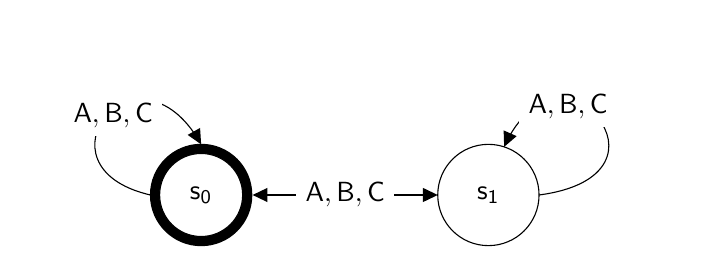
\begin{tikzpicture}[x=0.75pt,y=0.75pt,yscale=-0.8,xscale=0.8]
%uncomment if require: \path (0,150); %set diagram left start at 0, and has height of 150

%Shape: Circle [id:dp4325934269433842] 
\draw  [fill={rgb, 255:red, 0; green, 0; blue, 0 }  ,fill opacity=1 ] (216.5,93) .. controls (216.5,76.16) and (230.16,62.5) .. (247,62.5) .. controls (263.84,62.5) and (277.5,76.16) .. (277.5,93) .. controls (277.5,109.84) and (263.84,123.5) .. (247,123.5) .. controls (230.16,123.5) and (216.5,109.84) .. (216.5,93) -- cycle ;
%Shape: Circle [id:dp8959340303758652] 
\draw   (389.5,93) .. controls (389.5,76.16) and (403.16,62.5) .. (420,62.5) .. controls (436.84,62.5) and (450.5,76.16) .. (450.5,93) .. controls (450.5,109.84) and (436.84,123.5) .. (420,123.5) .. controls (403.16,123.5) and (389.5,109.84) .. (389.5,93) -- cycle ;
%Straight Lines [id:da6159546739572547] 
\draw    (280,93) -- (387.5,93) ;
\draw [shift={(389.5,93)}, rotate = 180] [fill={rgb, 255:red, 0; green, 0; blue, 0 }  ][line width=0.75]  [draw opacity=0] (8.93,-4.29) -- (0,0) -- (8.93,4.29) -- cycle    ;
\draw [shift={(278,93)}, rotate = 0] [fill={rgb, 255:red, 0; green, 0; blue, 0 }  ][line width=0.75]  [draw opacity=0] (8.93,-4.29) -- (0,0) -- (8.93,4.29) -- cycle    ;
%Curve Lines [id:da8452234444075793] 
\draw    (216.5,93) .. controls (142.87,76.08) and (207.84,-5.18) .. (246.42,61.48) ;
\draw [shift={(247,62.5)}, rotate = 240.66] [fill={rgb, 255:red, 0; green, 0; blue, 0 }  ][line width=0.75]  [draw opacity=0] (8.93,-4.29) -- (0,0) -- (8.93,4.29) -- cycle    ;

%Curve Lines [id:da8370233876099651] 
\draw    (450.5,93) .. controls (540.91,81.08) and (462.16,-7.43) .. (429.98,62.93) ;
\draw [shift={(429.5,64)}, rotate = 293.78] [fill={rgb, 255:red, 0; green, 0; blue, 0 }  ][line width=0.75]  [draw opacity=0] (8.93,-4.29) -- (0,0) -- (8.93,4.29) -- cycle    ;

%Shape: Circle [id:dp08152116050102409] 
\draw  [fill={rgb, 255:red, 255; green, 255; blue, 255 }  ,fill opacity=1 ] (222,93) .. controls (222,79.19) and (233.19,68) .. (247,68) .. controls (260.81,68) and (272,79.19) .. (272,93) .. controls (272,106.81) and (260.81,118) .. (247,118) .. controls (233.19,118) and (222,106.81) .. (222,93) -- cycle ;

% Text Node
\draw  [color={rgb, 255:red, 255; green, 255; blue, 255 }  ,draw opacity=1 ][fill={rgb, 255:red, 255; green, 255; blue, 255 }  ,fill opacity=1 ]  (304.75,81) -- (362.75,81) -- (362.75,105) -- (304.75,105) -- cycle  ;
\draw (333.75,93) node   {$\agent{A}, \agent{B}, \agent{C}$};
% Text Node
\draw (247,93) node   {$\defemph{s_0}$};
% Text Node
\draw (420,93) node   {$\defemph{s_1}$};
% Text Node
\draw  [color={rgb, 255:red, 255; green, 255; blue, 255 }  ,draw opacity=1 ][fill={rgb, 255:red, 255; green, 255; blue, 255 }  ,fill opacity=1 ]  (165,33) -- (223,33) -- (223,57) -- (165,57) -- cycle  ;
\draw (194,45) node   {$\agent{A}, \agent{B}, \agent{C}$};
% Text Node
\draw  [color={rgb, 255:red, 255; green, 255; blue, 255 }  ,draw opacity=1 ][fill={rgb, 255:red, 255; green, 255; blue, 255 }  ,fill opacity=1 ]  (439,28) -- (497,28) -- (497,52) -- (439,52) -- cycle  ;
\draw (468,40) node   {$\agent{A}, \agent{B}, \agent{C}$};

%\draw (340,160) node   {%
%	$\begin{aligned}
%	\interp{0}{s_0}&=\bra{\looking {AG}, \haskey A}\\
%	\interp{0}{s_1}&=\bra{\looking {AG}, \haskey{A}, \head}
%	\end{aligned}$
%	\hspace*{0.2cm}where \agent{ag} $\in$ \bra{\agent{a}, \agent{b}, \agent{c}}.};

\end{tikzpicture}


					}%
				}%
				\label{subfig-kripke:appendix_initial}
			}%
		\hspace*{.5cm}
			\subfloat[The initial \pos\ \poss{u}.]
			{% 
				\scalebox{0.95}%
				{%
					\raisebox{1.5cm}{
						
$\begin{cases}
 \poss u &= \bra{(\agentSlide{ag},\bra{\poss{u}, \poss{u^\prime}}),\\
 	&\text{~~~~~}\ttSlide{look(\agentSlide{ag})}, \ttSlide{key(\agentSlide{A})}, \ttSlide{heads}}\\
 \poss u^\prime &= \bra{(\agentSlide{ag},\bra{\poss{u}, \poss{u^\prime}}),\\
 	&\text{~~~~~}\ttSlide{look(\agentSlide{ag})}, \ttSlide{key(\agentSlide{A})}}
\end{cases}$

					}%
				}%
				\label{subfig-poss:appendix_initial}%
			}
			\caption{The initial state.}
			\label{fig:appendix_initial}
		\end{figure}%
%
		\begin{figure}[H]
			\centering
			\hspace*{-3cm}
			\subfloat[The Kripke stucture \state{1}{p_0}, obtained after the execution of \distract{C}{A}
			in \state{0}{s_0} (Figure~\ref{subfig-kripke:appendix_initial}).]
			{%
				\scalebox{.8}%
				{%
					\raisebox{0.5cm}{
						\input{img/distract_state_kripke}
					}%
				}%
				\label{subfig-kripke:appendix_distract}
			}%
			\hspace*{.5cm}
			\subfloat[\Pos\ \poss{v}, obtained after the execution of \distract{C}{A} in
			\poss{u} (Figure~\ref{subfig-poss:appendix_initial}).]
			{%
				\scalebox{0.95}%
				{%
					\raisebox{1.5cm}{
						$
\begin{aligned}
	&\begin{cases}
		\poss{v}&= \bra{
	     	(\agent{ag},\bra{\poss{v}, \poss{v^\prime}}),	\looking{a},
	     	\looking{b},
	     	\haskey{a}%
		}\\
			\poss{v}^\prime&= \bra{
	    	(\agent{ag},\bra{\poss{v}, \poss{v^\prime}}),
	    	\looking{a},
	    	\looking{b},
	    	\haskey{a},
	    	\head%
		}\\
	\end{cases}\\
	&\text{where }  \agent{ag}  \in \bra{\agent{A}, \agent{B}, \agent{C}}
\end{aligned}
$



					}%
				}%
				\label{subfig-poss:appendix_distract}%
			}
			\caption{Execution of \distract{C}{A}.}
			\label{fig:appendix_distract}
		\end{figure}%
%
		\begin{figure}[H]
			\centering
			\hspace*{-4cm}
			\subfloat[The Kripke stucture \state{2}{q_0}, obtained after the execution of \open{A}
			in \state{1}{p_0} (Figure~\ref{subfig-kripke:appendix_distract}).]
			{%
				\scalebox{.7}%
				{%
					\raisebox{0.0cm}{
						

\tikzset{every picture/.style={line width=0.75pt}} %set default line width to 0.75pt        

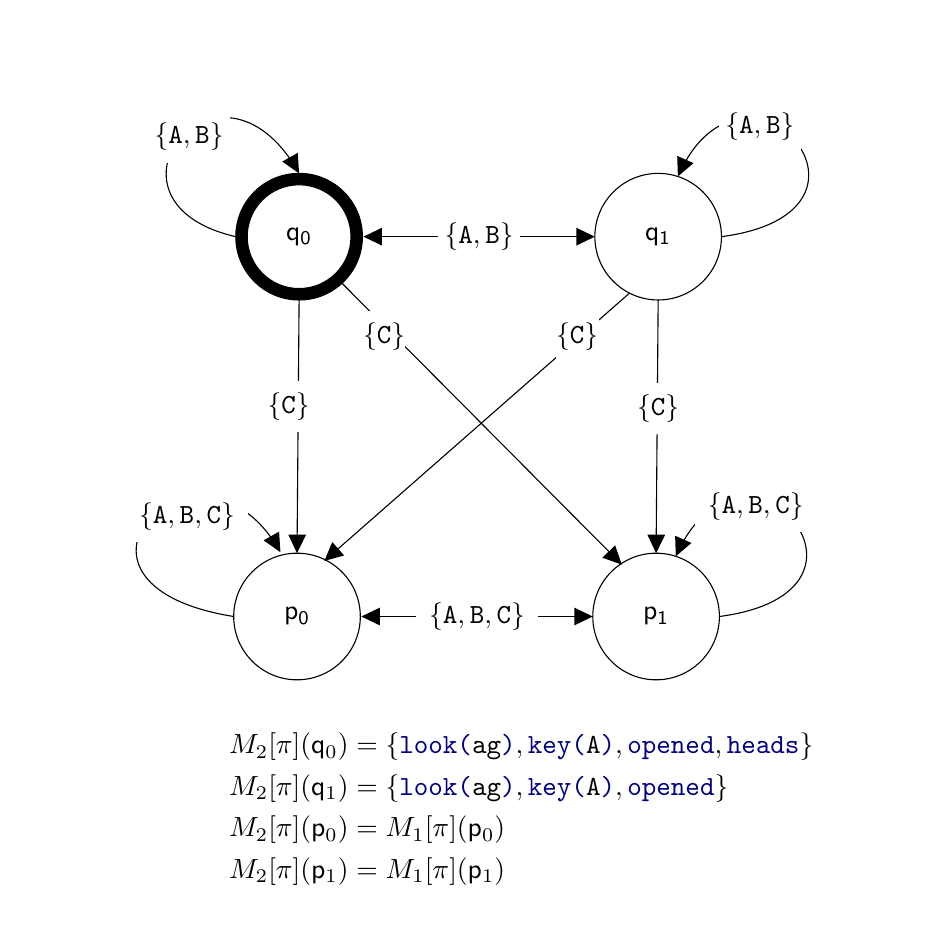
\begin{tikzpicture}[x=0.75pt,y=0.75pt,yscale=-1,xscale=1]
%uncomment if require: \path (0,371); %set diagram left start at 0, and has height of 371

%Shape: Circle [id:dp4325934269433842] 
\draw   (171.5,287) .. controls (171.5,270.16) and (185.16,256.5) .. (202,256.5) .. controls (218.84,256.5) and (232.5,270.16) .. (232.5,287) .. controls (232.5,303.84) and (218.84,317.5) .. (202,317.5) .. controls (185.16,317.5) and (171.5,303.84) .. (171.5,287) -- cycle ;
%Shape: Circle [id:dp8959340303758652] 
\draw   (344.5,287) .. controls (344.5,270.16) and (358.16,256.5) .. (375,256.5) .. controls (391.84,256.5) and (405.5,270.16) .. (405.5,287) .. controls (405.5,303.84) and (391.84,317.5) .. (375,317.5) .. controls (358.16,317.5) and (344.5,303.84) .. (344.5,287) -- cycle ;
%Straight Lines [id:da6159546739572547] 
\draw    (235,287) -- (342.5,287) ;
\draw [shift={(344.5,287)}, rotate = 180] [fill={rgb, 255:red, 0; green, 0; blue, 0 }  ][line width=0.75]  [draw opacity=0] (8.93,-4.29) -- (0,0) -- (8.93,4.29) -- cycle    ;
\draw [shift={(233,287)}, rotate = 0] [fill={rgb, 255:red, 0; green, 0; blue, 0 }  ][line width=0.75]  [draw opacity=0] (8.93,-4.29) -- (0,0) -- (8.93,4.29) -- cycle    ;
%Curve Lines [id:da8452234444075793] 
\draw    (171.5,287) .. controls (72.5,271.08) and (154.67,188.33) .. (193.42,254.98) ;
\draw [shift={(194,256)}, rotate = 240.66] [fill={rgb, 255:red, 0; green, 0; blue, 0 }  ][line width=0.75]  [draw opacity=0] (8.93,-4.29) -- (0,0) -- (8.93,4.29) -- cycle    ;

%Curve Lines [id:da8370233876099651] 
\draw    (405.5,287) .. controls (495.91,275.08) and (417.16,186.57) .. (384.98,256.93) ;
\draw [shift={(384.5,258)}, rotate = 293.78] [fill={rgb, 255:red, 0; green, 0; blue, 0 }  ][line width=0.75]  [draw opacity=0] (8.93,-4.29) -- (0,0) -- (8.93,4.29) -- cycle    ;

%Shape: Circle [id:dp7932635156571649] 
\draw  [fill={rgb, 255:red, 0; green, 0; blue, 0 }  ,fill opacity=1 ] (172.5,104) .. controls (172.5,87.16) and (186.16,73.5) .. (203,73.5) .. controls (219.84,73.5) and (233.5,87.16) .. (233.5,104) .. controls (233.5,120.84) and (219.84,134.5) .. (203,134.5) .. controls (186.16,134.5) and (172.5,120.84) .. (172.5,104) -- cycle ;
%Shape: Circle [id:dp6105058367437692] 
\draw   (345.5,104) .. controls (345.5,87.16) and (359.16,73.5) .. (376,73.5) .. controls (392.84,73.5) and (406.5,87.16) .. (406.5,104) .. controls (406.5,120.84) and (392.84,134.5) .. (376,134.5) .. controls (359.16,134.5) and (345.5,120.84) .. (345.5,104) -- cycle ;
%Straight Lines [id:da9340669325180512] 
\draw    (236,104) -- (343.5,104) ;
\draw [shift={(345.5,104)}, rotate = 180] [fill={rgb, 255:red, 0; green, 0; blue, 0 }  ][line width=0.75]  [draw opacity=0] (8.93,-4.29) -- (0,0) -- (8.93,4.29) -- cycle    ;
\draw [shift={(234,104)}, rotate = 0] [fill={rgb, 255:red, 0; green, 0; blue, 0 }  ][line width=0.75]  [draw opacity=0] (8.93,-4.29) -- (0,0) -- (8.93,4.29) -- cycle    ;
%Curve Lines [id:da4572197115547698] 
\draw    (172.5,104) .. controls (98.87,87.08) and (163.84,5.82) .. (202.42,72.48) ;
\draw [shift={(203,73.5)}, rotate = 240.66] [fill={rgb, 255:red, 0; green, 0; blue, 0 }  ][line width=0.75]  [draw opacity=0] (8.93,-4.29) -- (0,0) -- (8.93,4.29) -- cycle    ;

%Curve Lines [id:da9119172492888147] 
\draw    (406.5,104) .. controls (496.91,92.08) and (418.16,3.57) .. (385.98,73.93) ;
\draw [shift={(385.5,75)}, rotate = 293.78] [fill={rgb, 255:red, 0; green, 0; blue, 0 }  ][line width=0.75]  [draw opacity=0] (8.93,-4.29) -- (0,0) -- (8.93,4.29) -- cycle    ;

%Shape: Circle [id:dp47196260233615805] 
\draw  [fill={rgb, 255:red, 255; green, 255; blue, 255 }  ,fill opacity=1 ] (178,104) .. controls (178,90.19) and (189.19,79) .. (203,79) .. controls (216.81,79) and (228,90.19) .. (228,104) .. controls (228,117.81) and (216.81,129) .. (203,129) .. controls (189.19,129) and (178,117.81) .. (178,104) -- cycle ;
%Straight Lines [id:da04653031760639226] 
\draw    (222.75,125.5) -- (357.09,260.58) ;
\draw [shift={(358.5,262)}, rotate = 225.16] [fill={rgb, 255:red, 0; green, 0; blue, 0 }  ][line width=0.75]  [draw opacity=0] (8.93,-4.29) -- (0,0) -- (8.93,4.29) -- cycle    ;

%Straight Lines [id:da7004759142531133] 
\draw    (362.13,131.25) -- (216.63,258.93) ;
\draw [shift={(215.13,260.25)}, rotate = 318.73] [fill={rgb, 255:red, 0; green, 0; blue, 0 }  ][line width=0.75]  [draw opacity=0] (8.93,-4.29) -- (0,0) -- (8.93,4.29) -- cycle    ;

%Straight Lines [id:da7971203391650094] 
\draw    (203,134.5) -- (202.02,254.5) ;
\draw [shift={(202,256.5)}, rotate = 270.47] [fill={rgb, 255:red, 0; green, 0; blue, 0 }  ][line width=0.75]  [draw opacity=0] (8.93,-4.29) -- (0,0) -- (8.93,4.29) -- cycle    ;

%Straight Lines [id:da21593783196193417] 
\draw    (376,134.5) -- (375.02,254.5) ;
\draw [shift={(375,256.5)}, rotate = 270.47] [fill={rgb, 255:red, 0; green, 0; blue, 0 }  ][line width=0.75]  [draw opacity=0] (8.93,-4.29) -- (0,0) -- (8.93,4.29) -- cycle    ;


% Text Node
\draw  [color={rgb, 255:red, 255; green, 255; blue, 255 }  ,draw opacity=1 ][fill={rgb, 255:red, 255; green, 255; blue, 255 }  ,fill opacity=1 ]  (259.75,275) -- (317.75,275) -- (317.75,299) -- (259.75,299) -- cycle  ;
\draw (288.75,287) node   {\{$\agentSlide{A},\agentSlide{B},\agentSlide{C}$\}};
% Text Node
\draw (202,287) node   {\defemph{p_{0}}};
% Text Node
\draw (375,287) node   {\defemph{p_{1}}};
% Text Node
\draw  [color={rgb, 255:red, 255; green, 255; blue, 255 }  ,draw opacity=1 ][fill={rgb, 255:red, 255; green, 255; blue, 255 }  ,fill opacity=1 ]  (120,227) -- (178,227) -- (178,251) -- (120,251) -- cycle  ;
\draw (149,239) node   {\{$\agentSlide{A}, \agentSlide{B},\agentSlide{C}$\}};
% Text Node
\draw  [color={rgb, 255:red, 255; green, 255; blue, 255 }  ,draw opacity=1 ][fill={rgb, 255:red, 255; green, 255; blue, 255 }  ,fill opacity=1 ]  (394,222) -- (452,222) -- (452,246) -- (394,246) -- cycle  ;
\draw (423,234) node   {\{$\agentSlide{A},\agentSlide{B},\agentSlide{C}$\}};
% Text Node
\draw  [color={rgb, 255:red, 255; green, 255; blue, 255 }  ,draw opacity=1 ][fill={rgb, 255:red, 255; green, 255; blue, 255 }  ,fill opacity=1 ]  (270.25,92) -- (309.25,92) -- (309.25,116) -- (270.25,116) -- cycle  ;
\draw (289.75,104) node   {\{$\agentSlide{A},\agentSlide{B}$\}};
% Text Node
\draw (203,104) node   {\defemph{q_{0}}};
% Text Node
\draw (376,104) node   {\defemph{q_{1}}};
% Text Node
\draw  [color={rgb, 255:red, 255; green, 255; blue, 255 }  ,draw opacity=1 ][fill={rgb, 255:red, 255; green, 255; blue, 255 }  ,fill opacity=1 ]  (130.5,44) -- (169.5,44) -- (169.5,68) -- (130.5,68) -- cycle  ;
\draw (150,56) node   {\{$\agentSlide{A},\agentSlide{B}$\}};
% Text Node
\draw  [color={rgb, 255:red, 255; green, 255; blue, 255 }  ,draw opacity=1 ][fill={rgb, 255:red, 255; green, 255; blue, 255 }  ,fill opacity=1 ]  (405.5,39) -- (444.5,39) -- (444.5,63) -- (405.5,63) -- cycle  ;
\draw (425,51) node   {\{$\agentSlide{A},\agentSlide{B}$\}};
% Text Node
\draw  [color={rgb, 255:red, 255; green, 255; blue, 255 }  ,draw opacity=1 ][fill={rgb, 255:red, 255; green, 255; blue, 255 }  ,fill opacity=1 ]  (188,174) -- (208,174) -- (208,198) -- (188,198) -- cycle  ;
\draw (198,186) node   {\{$\agentSlide{C}$\}};
% Text Node
\draw  [color={rgb, 255:red, 255; green, 255; blue, 255 }  ,draw opacity=1 ][fill={rgb, 255:red, 255; green, 255; blue, 255 }  ,fill opacity=1 ]  (234,140) -- (254,140) -- (254,164) -- (234,164) -- cycle  ;
\draw (244,152) node   {\{$\agentSlide{C}$\}};
% Text Node
\draw  [color={rgb, 255:red, 255; green, 255; blue, 255 }  ,draw opacity=1 ][fill={rgb, 255:red, 255; green, 255; blue, 255 }  ,fill opacity=1 ]  (327,140) -- (347,140) -- (347,164) -- (327,164) -- cycle  ;
\draw (337,152) node   {\{$\agentSlide{C}$\}};
% Text Node
\draw  [color={rgb, 255:red, 255; green, 255; blue, 255 }  ,draw opacity=1 ][fill={rgb, 255:red, 255; green, 255; blue, 255 }  ,fill opacity=1 ]  (366,175) -- (386,175) -- (386,199) -- (366,199) -- cycle  ;
\draw (376,187) node   {\{$\agentSlide{C}$\}};

\draw (310,380) node   {
							$\begin{aligned}
							\interp{2}{q_0}&=\bra{\ttSlide{look(\agentSlide{ag})}, \ttSlide{key(\agentSlide{A})}, \ttSlide{opened}, \ttSlide{heads}}\\
							\interp{2}{q_1}&=\bra{\ttSlide{look(\agentSlide{ag})}, \ttSlide{key(\agentSlide{A})}, \ttSlide{opened}}\\
							\interp{2}{p_0}&=\interp{1}{p_0}\\
							\interp{2}{p_1}&=\interp{1}{p_1}
						\end{aligned}$};

\end{tikzpicture}


					}%
				}%
				\label{subfig-kripke:appendix_open}
			}%
			\hspace*{.5cm}
			\subfloat[\Pos\ \poss{w}, obtained after the execution of \open{A} in
			\poss{v} (Figure~\ref{subfig-poss:appendix_distract}).]
			{%
				\scalebox{0.95}%
				{%
					\raisebox{3.6cm}{
						$\begin{aligned}
  &\begin{cases}
    \poss{w}&= \bra{
      (\agentSlide{ag},\bra{\poss{w}, \poss{w^\prime}}),
      (\agentSlide{c},\bra{\poss{v}, \poss{v^\prime}}),\\
      &\text{~~~~~}\ttSlide{look(\agentSlide{ag})},
      \ttSlide{key(\agentSlide{A})},
      \ttSlide{opened}, \ttSlide{heads}}\\
    \poss{w^\prime} &=\bra{
      (\agentSlide{ag},\bra{\poss{w}, \poss{w^\prime}}),
      (\agentSlide{c},\bra{\poss{v}, \poss{v^\prime}}),\\
      &\text{~~~~~}\ttSlide{look(\agentSlide{ag})}, \ttSlide{key(\agentSlide{A})}, \ttSlide{opened}}
   \end{cases}\\
  &\text{where } \poss{v},
            \poss{v^\prime}, \text{ are defined as before}.
\end{aligned}$

					}%
				}%
				\label{subfig-poss:appendix_open}%
			}
			\caption{Execution of \open{A}.}
			\label{fig:appendix_open}
		\end{figure}%
%
		\begin{figure}[H]
			%\centering
			\hspace*{-4cm}
			\subfloat[The Kripke structure \state{3}{q_0}, obtained after the execution of \peek{A} in \state{2}{q_0}.]
			{%
				\scalebox{.7}%
				{%
					\raisebox{0.0cm}{
						\input{img/peek_state_kripke}
					}%
				}%
				\label{subfig-kripke:appendix_peek}
			}%
			\hspace*{.5cm}
			\subfloat[\Pos\ \poss{z}, obtained after the execution of \peek{A} in
			\poss{w} (Figure~\ref{subfig-poss:appendix_open}).]
			{% 
				\scalebox{0.95}%
				{%
					\raisebox{3.6cm}{
						$\begin{aligned}
&\begin{cases}
\poss{z} &= \bra{
	(\agentSlide{A},\bra{\poss{z}}), (\agentSlide{B}, \bra{\poss{z}, \poss{z^\prime}}) (\agentSlide{C}, \bra{\poss{v}, \poss{v^\prime}}),\\
	&\text{~~~~~}\ttSlide{look(\agentSlide{ag})},
	\ttSlide{key(\agentSlide{A})},
	\ttSlide{opened},
	\ttSlide{heads}}\\
\poss{z^\prime} &= \bra{
	(\agentSlide{A},\bra{\poss{z^\prime}}), (\agentSlide{B}, \bra{\poss{z}, \poss{z^\prime}}) (\agentSlide{C}, \bra{\poss{v}, \poss{v^\prime}}),\\
	&\text{~~~~~}\ttSlide{look(\agentSlide{ag})},
	\ttSlide{key(\agentSlide{A})},
	\ttSlide{opened},}
\end{cases}\\
&\text{where the \posS\ \poss{v}, \poss{v^\prime} are defined as before.}
\end{aligned}$



					}%
				}%
				\label{subfig-poss:appendix_peek}%
			}
			\caption{Execution of \peek{A}.}
			\label{fig:appendix_peek}
		\end{figure}%
%	
%		Both the state in Figure~\ref{fig:appendix_peek} entail the desired goal that is expressed with the following formulae:
%		\begin{align*}
%			&\bB{A}{\neg \head} \wedge \bB{A}{(\bB{B}{(\bB{A}{\head}
%				\vee \bB{A}{\neg \head})})}\\
%			&\bB{B}{(\bB{A}{\head}\vee \bB{A}{\neg \head})} \wedge
%			(\neg \bB{B}{\head \wedge \neg \bB{B}{\neg \head}})\\
%			&\bB{C}[\bigwedge_{\agent{AG} \in \bra{\agent A, \agent B, \agent C}}(\neg\bB{ag}{\head}
%			\wedge \neg\bB{ag}{\neg \head}) ]
%		%	\state{3}{z_0} &\models\,C_{\bra{\agent A, \agent B}}(\neg\bB{B}{\head} \wedge \neg \bB{B}{\head)}
%		\end{align*}
%		\begin{align*}
%			\state{3}{z_0} &\models \bB{A}{\neg \head} \wedge \bB{A}{(\bB{B}{(\bB{A}{\head}
%					\vee \bB{A}{\neg \head})})}\\
%			\state{3}{z_0} &\models \bB{B}{(\bB{A}{\head}\vee \bB{A}{\neg \head})} \wedge
%			(\neg \bB{B}{\head \wedge \neg \bB{B}{\neg \head}})\\
%			\state{3}{z_0} &\models \bB{C}[\bigwedge_{\agent{AG} \in \bra{\agent A, \agent B, \agent C}}(\neg\bB{ag}{\head}
%			\wedge \neg\bB{ag}{\neg \head}) ]
%		%	\state{3}{z_0} &\models\,C_{\bra{\agent A, \agent B}}(\neg\bB{B}{\head} \wedge \neg \bB{B}{\head)}
%		\end{align*}
	
\end{document}
